\documentclass[declaration,shortabstract,english,mgr]{iithesis}

\usepackage[automake, acronym, nonumberlist, nopostdot]{glossaries}

\usepackage{cite}
\usepackage{hyperref}
\usepackage{listings}
\usepackage{graphicx}
\usepackage[T1]{fontenc}
\usepackage[utf8]{inputenc}
\usepackage{proof}
\usepackage{amsmath}
\usepackage{savesym}
\savesymbol{lll}
\usepackage{amssymb}
\usepackage{wasysym}

\graphicspath{ {./img/} }

\lstset
{
	basicstyle=\small\ttfamily,
	frame=bt,
	numbers=left,
	tabsize=2,
	captionpos=b,
	aboveskip=2em,
	belowskip=2em,
	breaklines=true
}

\polishtitle    {Implementacja i testowanie \fmlinebreak interpretera języka CIL}
\englishtitle   {Implementation and testing \fmlinebreak of the CIL interpreter}
\author         {Kamil Kwaśny}
\advisor        {dr Wiktor Zychla}

\polishabstract {\ldots}
\englishabstract{\ldots}

%%%%%%%%%%%%%%%%%%%%%%%%%%%%%%%%%%%%%%%%%%%%%%%%%%%%%%%%%%%%%%%%%%%%%%%%%%%%%%%%%%%%%%%%%%
%%%%%%%%%%%%%%%%%%%%%%%%%%%%%%%%%%%%%%%%%%%%%%%%%%%%%%%%%%%%%%%%%%%%%%%%%%%%%%%%%%%%%%%%%%
%%%%%
%%%%%	Commands
%%%%%
%%%%%%%%%%%%%%%%%%%%%%%%%%%%%%%%%%%%%%%%%%%%%%%%%%%%%%%%%%%%%%%%%%%%%%%%%%%%%%%%%%%%%%%%%%
%%%%%%%%%%%%%%%%%%%%%%%%%%%%%%%%%%%%%%%%%%%%%%%%%%%%%%%%%%%%%%%%%%%%%%%%%%%%%%%%%%%%%%%%%%
		
\renewcommand{\lstlistingname}{Code listing}
\renewcommand{\lstlistlistingname}{List of code listings}

\newcommand{\mstate}[5] {
	\langle#1, #2, #3, #4, #5\rangle
}

\newcommand{\ipointsto}[3] {
	#1 \leadsto \texttt{#2} \text{ } #3
}

\newcommand{\sval}[2] {
	#1_\texttt{#2}
}

\newcommand{\setarrayitem}[3] {
	#1[#2 \mapsto #3]
}

%%%%%%%%%%%%%%%%%%%%%%%%%%%%%%%%%%%%%%%%%%%%%%%%%%%%%%%%%%%%%%%%%%%%%%%%%%%%%%%%%%%%%%%%%%
%%%%%%%%%%%%%%%%%%%%%%%%%%%%%%%%%%%%%%%%%%%%%%%%%%%%%%%%%%%%%%%%%%%%%%%%%%%%%%%%%%%%%%%%%%
%%%%%
%%%%%	Create acronyms
%%%%%
%%%%%%%%%%%%%%%%%%%%%%%%%%%%%%%%%%%%%%%%%%%%%%%%%%%%%%%%%%%%%%%%%%%%%%%%%%%%%%%%%%%%%%%%%%
%%%%%%%%%%%%%%%%%%%%%%%%%%%%%%%%%%%%%%%%%%%%%%%%%%%%%%%%%%%%%%%%%%%%%%%%%%%%%%%%%%%%%%%%%%

\newacronym{cil}{CIL}{Common Intermediate Language}
\newacronym{msil}{MSIL}{Microsoft Intermediate Language}
\newacronym{il}{IL}{Intermediate Language}
\newacronym{cli}{CLI}{Common Language Infrastructure}
\newacronym{iso}{ISO}{International Organization for Standardization}
\newacronym{cts}{CTS}{Common Type System}
\newacronym{cls}{CLS}{Common Language Specification}
\newacronym{ves}{VES}{Virtual Execution System}
\newacronym{ast}{AST}{Abstract syntax tree}
\makeglossaries

%%%%%%%%%%%%%%%%%%%%%%%%%%%%%%%%%%%%%%%%%%%%%%%%%%%%%%%%%%%%%%%%%%%%%%%%%%%%%%%%%%%%%%%%%%
%%%%%%%%%%%%%%%%%%%%%%%%%%%%%%%%%%%%%%%%%%%%%%%%%%%%%%%%%%%%%%%%%%%%%%%%%%%%%%%%%%%%%%%%%%
%%%%%
%%%%%	Begin document
%%%%%
%%%%%%%%%%%%%%%%%%%%%%%%%%%%%%%%%%%%%%%%%%%%%%%%%%%%%%%%%%%%%%%%%%%%%%%%%%%%%%%%%%%%%%%%%%
%%%%%%%%%%%%%%%%%%%%%%%%%%%%%%%%%%%%%%%%%%%%%%%%%%%%%%%%%%%%%%%%%%%%%%%%%%%%%%%%%%%%%%%%%%

\begin{document}

%%%%%%%%%%%%%%%%%%%%%%%%%%%%%%%%%%%%%%%%%%%%%%%%%%%%%%%%%%%%%%%%%%%%%%%%%%%%%%%%%%%%%%%%%%
%%%%%%%%%%%%%%%%%%%%%%%%%%%%%%%%%%%%%%%%%%%%%%%%%%%%%%%%%%%%%%%%%%%%%%%%%%%%%%%%%%%%%%%%%%
%%%%%
%%%%%	Acronyms
%%%%%
%%%%%%%%%%%%%%%%%%%%%%%%%%%%%%%%%%%%%%%%%%%%%%%%%%%%%%%%%%%%%%%%%%%%%%%%%%%%%%%%%%%%%%%%%%
%%%%%%%%%%%%%%%%%%%%%%%%%%%%%%%%%%%%%%%%%%%%%%%%%%%%%%%%%%%%%%%%%%%%%%%%%%%%%%%%%%%%%%%%%%

\printglossary[type=\acronymtype]

%%%%%%%%%%%%%%%%%%%%%%%%%%%%%%%%%%%%%%%%%%%%%%%%%%%%%%%%%%%%%%%%%%%%%%%%%%%%%%%%%%%%%%%%%%
%%%%%%%%%%%%%%%%%%%%%%%%%%%%%%%%%%%%%%%%%%%%%%%%%%%%%%%%%%%%%%%%%%%%%%%%%%%%%%%%%%%%%%%%%%
%%%%%
%%%%%	Figures
%%%%%
%%%%%%%%%%%%%%%%%%%%%%%%%%%%%%%%%%%%%%%%%%%%%%%%%%%%%%%%%%%%%%%%%%%%%%%%%%%%%%%%%%%%%%%%%%
%%%%%%%%%%%%%%%%%%%%%%%%%%%%%%%%%%%%%%%%%%%%%%%%%%%%%%%%%%%%%%%%%%%%%%%%%%%%%%%%%%%%%%%%%%

\listoffigures

%%%%%%%%%%%%%%%%%%%%%%%%%%%%%%%%%%%%%%%%%%%%%%%%%%%%%%%%%%%%%%%%%%%%%%%%%%%%%%%%%%%%%%%%%%
%%%%%%%%%%%%%%%%%%%%%%%%%%%%%%%%%%%%%%%%%%%%%%%%%%%%%%%%%%%%%%%%%%%%%%%%%%%%%%%%%%%%%%%%%%
%%%%%
%%%%%	List of tables
%%%%%
%%%%%%%%%%%%%%%%%%%%%%%%%%%%%%%%%%%%%%%%%%%%%%%%%%%%%%%%%%%%%%%%%%%%%%%%%%%%%%%%%%%%%%%%%%
%%%%%%%%%%%%%%%%%%%%%%%%%%%%%%%%%%%%%%%%%%%%%%%%%%%%%%%%%%%%%%%%%%%%%%%%%%%%%%%%%%%%%%%%%%

\listoftables

%%%%%%%%%%%%%%%%%%%%%%%%%%%%%%%%%%%%%%%%%%%%%%%%%%%%%%%%%%%%%%%%%%%%%%%%%%%%%%%%%%%%%%%%%%
%%%%%%%%%%%%%%%%%%%%%%%%%%%%%%%%%%%%%%%%%%%%%%%%%%%%%%%%%%%%%%%%%%%%%%%%%%%%%%%%%%%%%%%%%%
%%%%%
%%%%%	Code listings
%%%%%
%%%%%%%%%%%%%%%%%%%%%%%%%%%%%%%%%%%%%%%%%%%%%%%%%%%%%%%%%%%%%%%%%%%%%%%%%%%%%%%%%%%%%%%%%%
%%%%%%%%%%%%%%%%%%%%%%%%%%%%%%%%%%%%%%%%%%%%%%%%%%%%%%%%%%%%%%%%%%%%%%%%%%%%%%%%%%%%%%%%%%

\lstlistoflistings

%%%%%%%%%%%%%%%%%%%%%%%%%%%%%%%%%%%%%%%%%%%%%%%%%%%%%%%%%%%%%%%%%%%%%%%%%%%%%%%%%%%%%%%%%%
%%%%%%%%%%%%%%%%%%%%%%%%%%%%%%%%%%%%%%%%%%%%%%%%%%%%%%%%%%%%%%%%%%%%%%%%%%%%%%%%%%%%%%%%%%
%%%%%
%%%%%	Introduction
%%%%%
%%%%%%%%%%%%%%%%%%%%%%%%%%%%%%%%%%%%%%%%%%%%%%%%%%%%%%%%%%%%%%%%%%%%%%%%%%%%%%%%%%%%%%%%%%
%%%%%%%%%%%%%%%%%%%%%%%%%%%%%%%%%%%%%%%%%%%%%%%%%%%%%%%%%%%%%%%%%%%%%%%%%%%%%%%%%%%%%%%%%%

\chapter{Introduction}

\section{The \acrlong{cli}}

\textit{The \acrfull{cli}} is a specification developed by \textit{Microsoft} and standardized by \textit{\acrshort{iso}} and \textit{ECMA International} \cite{isoStandard, ecmaStandard}. It describes executable code and an environment that allows numerous programming languages to be executed on various platforms.

The following four main aspects are covered by the \acrlong{cli} \cite{ecmaStandard}:
\begin{itemize}
	\item{
		\textbf{\textit{The \acrfull{cts}}} - a type system supporting types and operations found in many programming languages;
	}
	\item{
		\textbf{Metadata} - used for describing and referencing types defined by the \acrshort{cts};
	}
	\item{
		\textbf{\textit{The \acrfull{cls}}} - an agreement between language designers and framework designers specifying a subset of the \acrshort{cts} and a set of usage conventions;
	}
	\item{
		\textbf{\textit{The \acrfull{ves}}} - responsible for loading and executing programs written for the \acrshort{cli}.
	}
\end{itemize}

There are multiple implementations of the \acrshort{cli}, for instance: \textit{.NET Framework}, \textit{Shared Source Common Language Infrastructure Implementation}, \textit{.NET Core} and \textit{Mono}.

\section{The \acrlong{cil}}

\textit{The \acrfull{cil}} is also known as \textit{the \acrfull{msil}} or simply \textit{the \acrfull{il}} \cite{procsharp7}. It is an object-oriented programming language that is a part of the \acrshort{cli}. Each language compatible with the \acrshort{cli} is compiled into the \acrshort{cil}. Moreover, the \acrshort{cil} is the actual language executed by the \acrshort{ves}. The language is a reasonable compromise between user-friendly, high-level programming languages and low-level assemblers. Although the \acrshort{cil} is human-readable, it is still a stack-based language and writing programs manually is therefore quite difficult.

Technically, the \acrshort{cil} is just a set of over 200 instructions and it does not define a syntax for describing \textit{the \acrshort{cli} metadata}. There is another syntax called \textit{ILAsm} - an assembly language for the \acrshort{cil} \cite{ecmaStandard}. However, many sources refer to the \acrshort{cil} and ILAsm interchangeably. Thus, \textit{the \acrshort{cil}} means hereinafter the whole ILAsm syntax and \textit{the \acrshort{cil} instruction set} refers to the correct meaning of the \acrlong{cil}.

\begin{lstlisting}[
	caption={\textit{Hello world} program.},
	label={lst:hello_world}
]
.assembly extern mscorlib {}

.assembly HelloWorld {}

.method static public void main() cil managed
{
	.entrypoint
	.maxstack 1
	ldstr "Hello world!"
	call void [mscorlib]System.Console::WriteLine(string)
	ret
}
\end{lstlisting}

The difference between ILAsm and the \acrshort{cil} can be easily understood by analysing the \textit{Hello world} program shown in code listing \ref{lst:hello_world}. Lines 1-8 and 12 of the example contain the \acrshort{cli} metadata described in ILasm syntax whereas lines 9-11 contain actual \acrshort{cil} instructions. The detailed meaning of each line can be explained as follows:
\begin{itemize}
	\item{Line 1 informs that an external assembly (\texttt{mscorlib}) should be loaded.}
	\item{Line 3 defines the assembly that should be created as the result of the compiler.}
	\item{Line 5 declares a static public method (\texttt{main}). It also defines that the method contains \acrshort{cil} code.}
	\item{Line 6 begins the body of the \texttt{main} method.}
	\item{Line 7 informs that the method should be used as the entry point of the program - it should be called by the compiler as the very first method.}
	\item{Line 8 specifies the maximal size of the evaluation stack associated with the method.}
	\item{Line 9 contains a \texttt{ldstr} instruction. It tells the compiler to put the \textit{Hello world!} string onto the evaluation stack.}
	\item{Line 10 contains a \texttt{call} instruction. It tells the compiler to call the \texttt{WriteLine} method from the \texttt{System.Console} class defined in the \texttt{mscorlib} assembly.}
	\item{Line 11 contains a \texttt{ret} instruction. It tells the compiler to return the result of the method and to transfer the control to the next method on the call stack.}
	\item{Line 12 ends the body of the \texttt{main} method.}
\end{itemize}

\section{Thesis motivation and organisation}

Being a student of Computer Science and working as a \texttt{C\#} and \texttt{.NET} developer for several years was an inspiration that resulted in this very thesis. It focuses on some fundamental and theoretical aspects of the \acrshort{cil} and particularly on the \acrshort{cil} instruction set. There are 3 goals of the thesis:
\begin{itemize}
	\item{investigate the semantics of the \acrshort{cil},}
	\item{implement an interpreter of the \acrshort{cil} covering various instructions,}
	\item{create a comprehensive environment for testing the interpreter.}
\end{itemize}

The main concepts of the \acrshort{cil} instructions are presented in chapter \ref{sec:instructionSet}. Chapter \ref{sec:semantics} introduces a formal mathematical model and tries to specify the semantics of the \acrshort{cil}. The interpreter together with its technical details is described in chapter \ref{sec:interpreter}. The environment and the methodology of testing are presented in chapter \ref{sec:testing}. Chapter \ref{sec:results} summarises the results while chapter \ref{sec:conclusions} contains the conclusions and suggests some ideas that could be potentially undertaken in the future.

All the source code produced as a part of the thesis can be found in the repository available under the following link:
\begin{center}
	\href{https://github.com/kvasnyk/CILantro}{\texttt{https://github.com/kvasnyk/CILantro}}.
\end{center}

\clearpage

%%%%%%%%%%%%%%%%%%%%%%%%%%%%%%%%%%%%%%%%%%%%%%%%%%%%%%%%%%%%%%%%%%%%%%%%%%%%%%%%%%%%%%%%%%
%%%%%%%%%%%%%%%%%%%%%%%%%%%%%%%%%%%%%%%%%%%%%%%%%%%%%%%%%%%%%%%%%%%%%%%%%%%%%%%%%%%%%%%%%%
%%%%%
%%%%%	The CIL instruction set
%%%%%
%%%%%%%%%%%%%%%%%%%%%%%%%%%%%%%%%%%%%%%%%%%%%%%%%%%%%%%%%%%%%%%%%%%%%%%%%%%%%%%%%%%%%%%%%%
%%%%%%%%%%%%%%%%%%%%%%%%%%%%%%%%%%%%%%%%%%%%%%%%%%%%%%%%%%%%%%%%%%%%%%%%%%%%%%%%%%%%%%%%%%

\chapter{The CIL instruction set}
\label{sec:instructionSet}

In order to understand how the \acrshort{cil} instructions work, this chapter explains the concept of the global state and provides code examples introducing several \acrshort{cil} instructions. As the whole set contains more than 200 instructions, further information on each of them can be found in \cite{ecmaStandard} and \cite{isoStandard}. A full list of the instructions is also shown in tables \ref{tab:coverage1} and \ref{tab:coverage2} which illustrate whether each instruction was implemented in the final interpreter or not.

\section{The global state}
\label{sec:global_state}

The \acrshort{cli} can manage multiple threads of control at the same time. A single thread of control can be thought as a call stack consisting of multiple method states. Although all the threads of control are rather independent, they still can access multiple managed heaps allocated in the shared memory space \cite{ecmaStandard}. This concept is presented in figure \ref{fig:global_state}.

\begin{figure}
	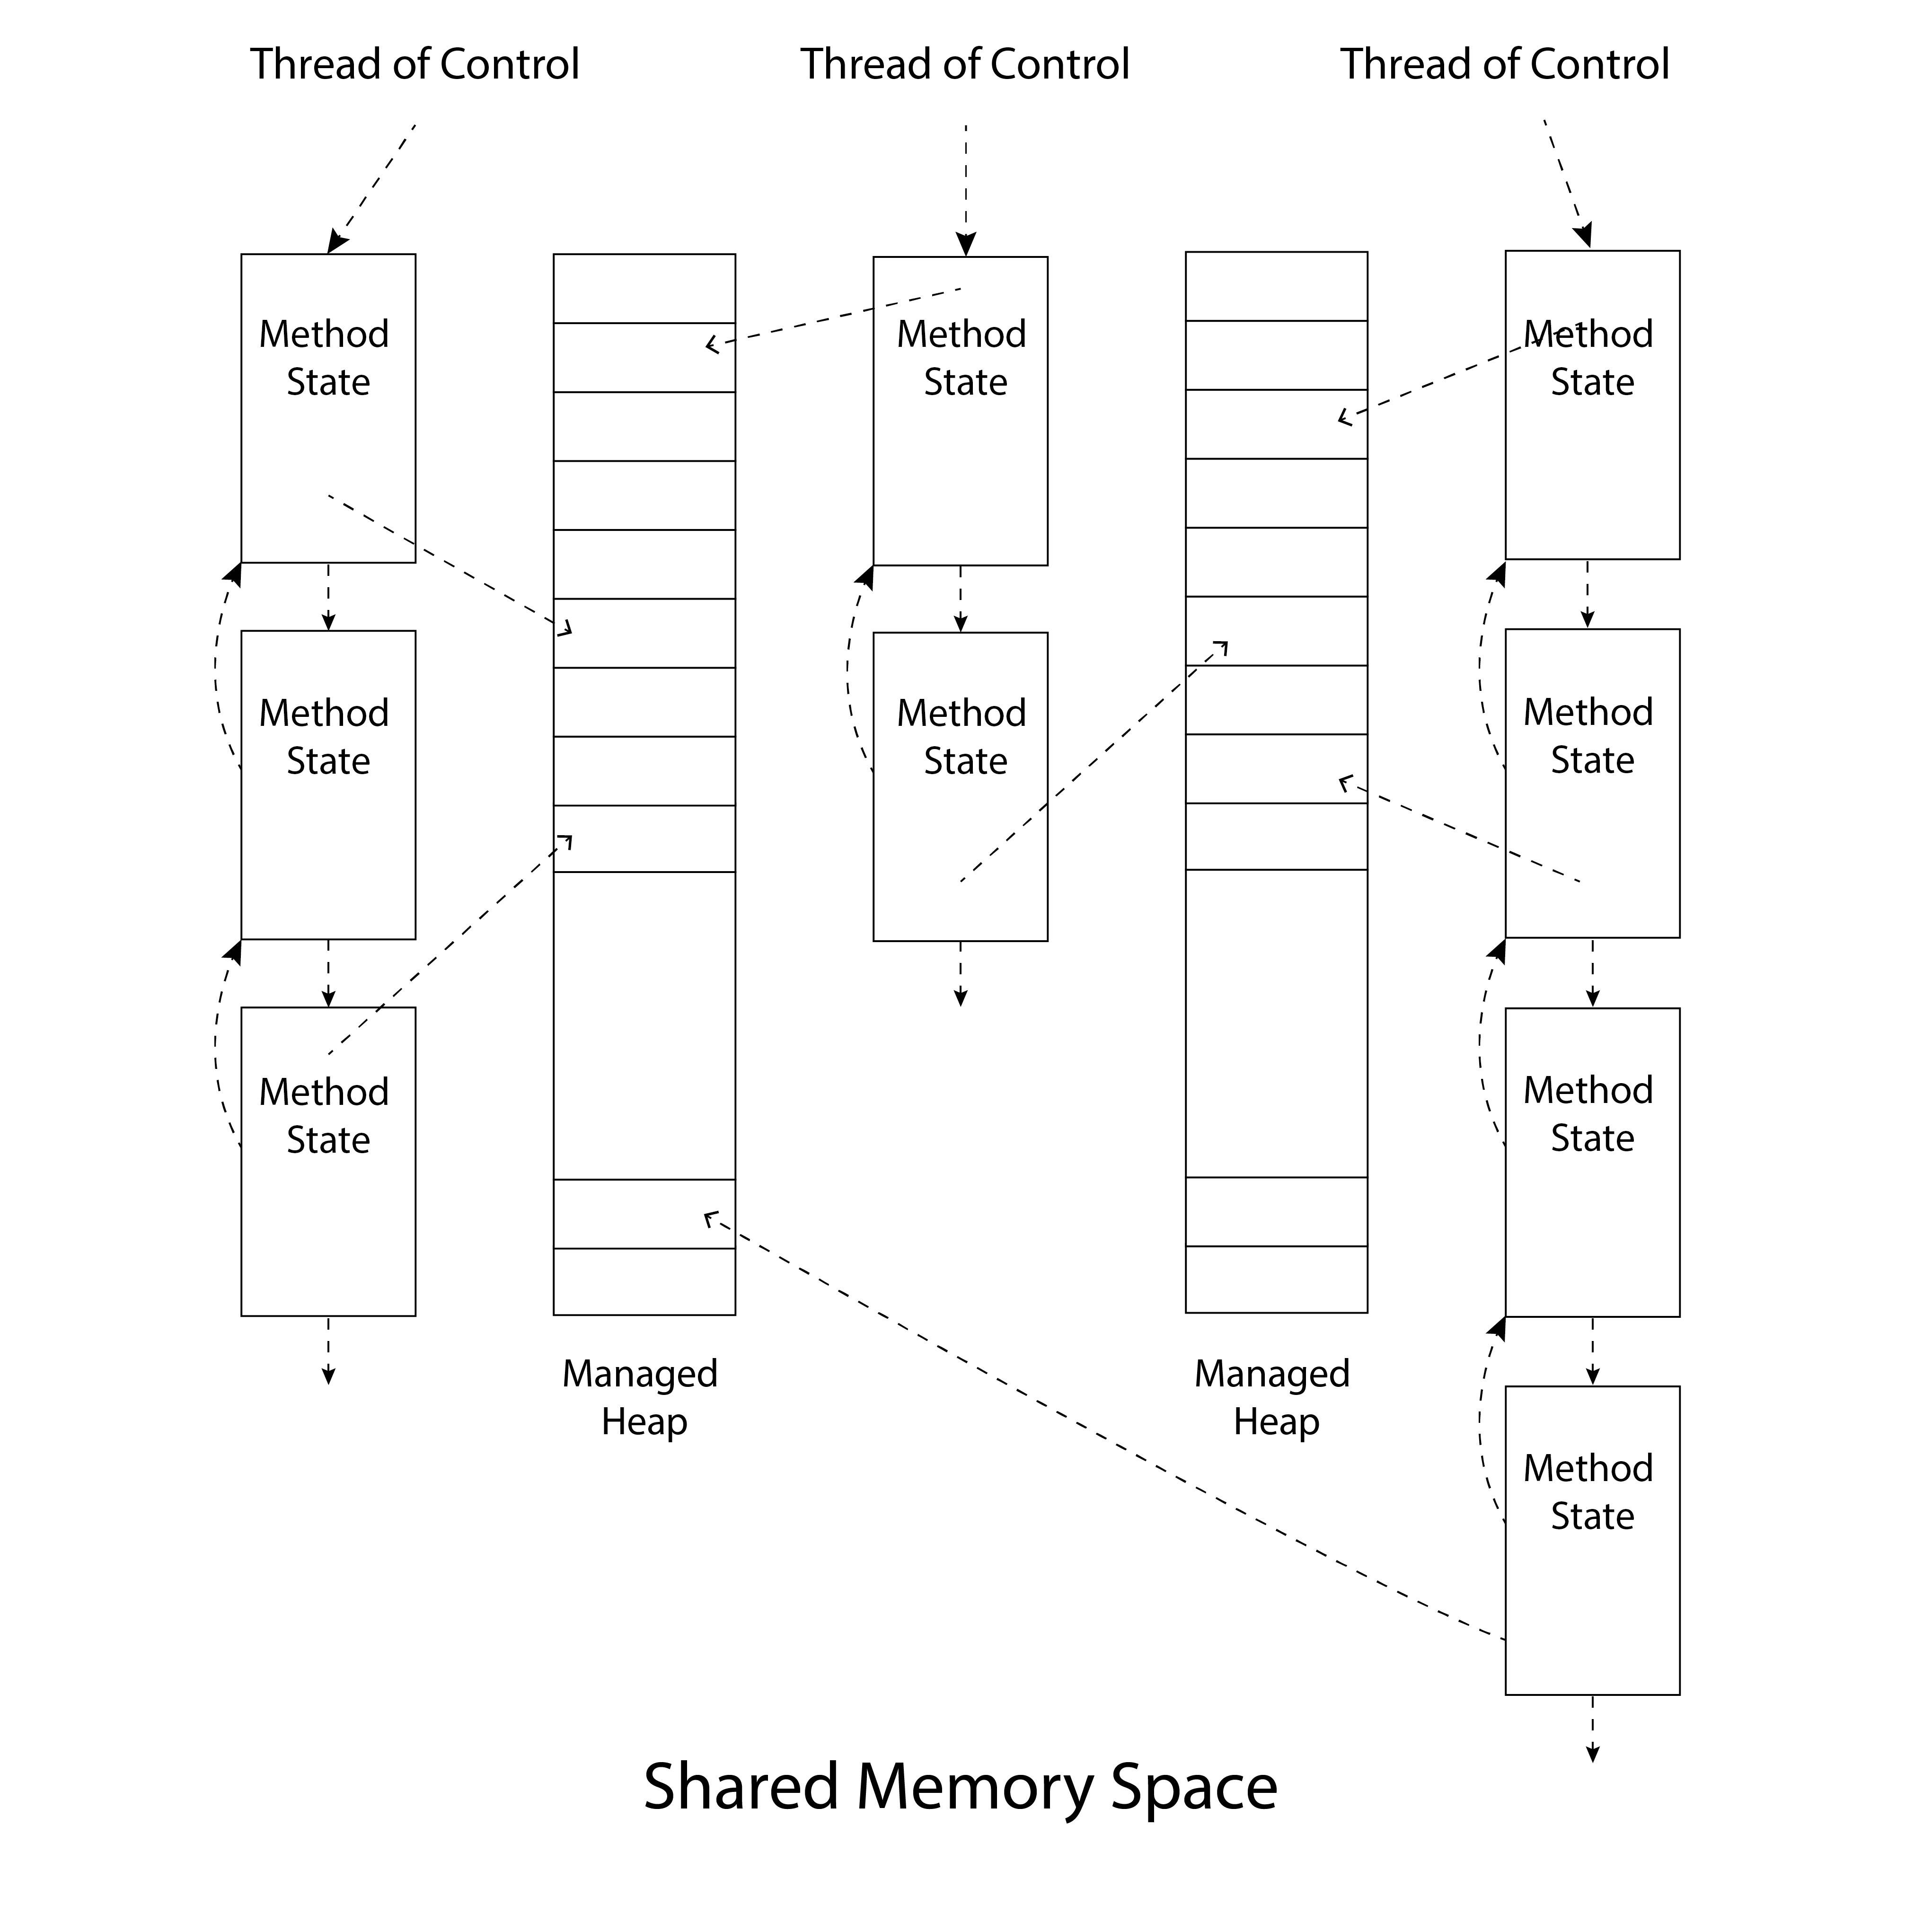
\includegraphics[width=1\textwidth]{global_state.png}
    \centering
    \caption{The global state concept.}
    \label{fig:global_state}
\end{figure}

A single method state includes several items required for the \acrshort{ves} to execute the method \cite{ecmaStandard}, inter alia:
\begin{itemize}
	\item{an instruction pointer - it determines the next instruction that should be executed within the method;}
	\item{an evaluation stack - it stores evaluation values;}
	\item{a method information handle - it contains read-only method information;}
	\item{a local variable array;}
	\item{an argument array.}
\end{itemize}

Generally, a single instruction can be understood as a description of how to manipulate the corresponding method state - there are only a few exceptions to this rule. Some instructions only require access to the evaluation stack while some do need to change other parts of the global state. To better understand these differences, the examples below present a couple of instructions and describe what effect they have on the global state.

\section{The evaluation stack}

As described above, a method state contains an evaluation stack. While a rich set of data types can be represented in memory, only a very limited subset of those types are supported by the \acrshort{cli} on an evaluation stack. This subset consists of the following data types \cite{ecmaStandard}:
\begin{itemize}
	\item{\texttt{int32},}
	\item{\texttt{int64},}
	\item{\texttt{native int},}
	\item{\texttt{F} (a floating-point number),}
	\item{\texttt{O} (an object reference),}
	\item{\texttt{\&} (a managed pointer),}
	\item{\texttt{native unsigned int} (also an unmanaged pointer),}
	\item{a user-defined value type.}
\end{itemize}

\section{Stack transformations}
\label{sec:stackTransformations}

A stack transformation can be thought as a sequence of pop and / or push operations performed on an evaluation stack. The majority of the \acrshort{cil} instructions uses such a sequence to get some values from the corresponding stack or to push some values onto it. In order to describe and visualise the effect of an instruction, the following syntax is used:
\begin{itemize}
	\item{$S$ denotes an evaluation stack;}
	\item{$S \rightarrow S \cdot v_1 \cdot v_2 \cdot ... \cdot v_n$ denotes a stack transformation which is equivalent to pushing the values $v_1, v_2, ..., v_n$ onto the stack $S$;}
	\item{$S \cdot u_1 \cdot u_2 \cdot ... \cdot u_n \rightarrow S$ denotes a stack transformation which is equivalent to popping the values $u_1, u_2, ..., u_n$ from the stack $S$;}
	\item{$S \cdot u_1 \cdot u_2 \cdot ... \cdot u_n \rightarrow S \cdot v_1 \cdot v_2 \cdot ... \cdot v_m$ denotes a stack transformation which is equivalent to popping values $u_1, u_2, ..., u_n$ from the stack $S$ and then pushing the values $v_1, v_2, ..., v_m$ onto it.}
\end{itemize}

\section{Stack values}

To illustrate the difference between various stack values, the following syntax represents the value $v$ of the stack type \texttt{type}:
$$
	\sval{v}{type}
$$.
For instance, $\sval{0}{int32}$ represents $0$ of type \texttt{int32}.

\section{Examples}
\label{sec:instruction_examples}

\subsection{\texttt{ldc.i4.0}}
\label{sec:desc_ldci40}

The \texttt{ldc.i4.0} instruction pushes $0$ onto the evaluation stack as \texttt{int32}. The corresponding stack transformation can be presented as follows \cite{ecmaStandard}:
$$
	S \rightarrow S \cdot 0_\texttt{int32}
$$

The program shown in code listing \ref{lst:ldci40} uses the instruction to push $0$ onto the stack and then writes out the top stack value ($0$) using the \texttt{call} instruction.

\begin{lstlisting}[
	caption={Usage of the \texttt{ldc.i4.0} instruction.},
	label={lst:ldci40}
]
.assembly extern mscorlib {}

.assembly HelloWorld {}

.method static public void main() cil managed
{
	.entrypoint
	.maxstack 1
	ldc.i4.0
	call void [mscorlib]System.Console::WriteLine(int32)
	ret
}
\end{lstlisting}

The \acrshort{cil} provides a number of similar instructions to push other constant values onto the stack: \texttt{ldc.i4.1}, \texttt{ldc.i4.2}, \texttt{ldc.i4.3}, \texttt{ldc.i4.4}, \texttt{ldc.i4.5}, \texttt{ldc.i4.6}, \texttt{ldc.i4.7}, \texttt{ldc.i4.8} and \texttt{ldc.i4.m1} (or \texttt{ldc.i4.M1}) which pushes $-1$ onto the stack.

\subsection{\texttt{stloc.0} and \texttt{ldloc.0}}
\label{sec:desc_stloc0_ldloc0}

The \texttt{stloc.0} instruction pops a value $v$ from the evaluation stack and moves it to the $0$-th position in the local variable array. Its stack transformation can be represented as follows \cite{ecmaStandard}:
$$
	S \cdot v \rightarrow S
$$

Conversely, the \texttt{ldloc.0} instruction loads the $0$-th local variable $v$ onto the evaluation stack and its stack transformation is \cite{ecmaStandard}:
$$
	S \rightarrow S \cdot v
$$

The program shown in code listing \ref{lst:stloc0_ldloc0} uses both instruction to store $7$ in the $0$-th local variable and then to load it onto the stack.

There are several similar instructions provided by the \acrshort{cil}: \texttt{stloc.1}, \texttt{stloc.2}, \texttt{stloc.3}, \texttt{stloc}, \texttt{stloc.s}, \texttt{ldloc.1}, \texttt{ldloc.2}, \texttt{ldloc.3}, \texttt{ldloc}, \texttt{ldloc.s}.

\begin{lstlisting}[
	caption={Usage of the \texttt{stloc.0} and \texttt{ldloc.0} instructions.},
	label={lst:stloc0_ldloc0}
]
.assembly extern mscorlib {}

.assembly HelloWorld {}

.method static public void main() cil managed
{
	.entrypoint
	.maxstack 1
	.locals init ([0] int32 n)
	ldc.i4.7
	stloc.0
	ldloc.0
	call void [mscorlib]System.Console::WriteLine(int32)
	ret
}
\end{lstlisting}

\subsection{\texttt{add}}

The \texttt{add} instruction is responsible for adding 2 numeric values so its stack transformation is as follows \cite{ecmaStandard}:
$$
	S, v_1, v_2 \rightarrow S, r
$$
where $r = v_1 + v_2$. The instruction does not detect any overflows and its result type is computed based on the types of $v_1$ and $v_2$. For instance:
\begin{itemize}
	\item{If $v_1$ is \texttt{int32} and $v_2$ is \texttt{int32}, the result type is also \texttt{int32}.}
	\item{If $v_1$ is \texttt{int64} and $v_2$ is \texttt{int64}, the result type is also \texttt{int64}.}
	\item{If $v_1$ is \texttt{int32} and $v_2$ is \texttt{int64}, the operation is invalid. However, it seems the \texttt{.NET} implementation of the \acrshort{cli} does not respect this part of the documentation as it allows adding (and other binary numeric operations) for values of types \texttt{int32} and \texttt{int64}.}
\end{itemize}
The full table of valid combinations of $v_1$ and $v_2$ types with their result types can be found in \cite{ecmaStandard}. It applies to various binary numeric operations such as \texttt{sub}, \texttt{mul} and \texttt{div}.

The example presented in listing \ref{lst:add} pushes 2 and 7 onto the stack, adds them using the \texttt{add} instruction and writes out the result to the console.

\begin{lstlisting}[
	caption={Usage of the \texttt{add} instruction.},
	label={lst:add}
]
.assembly extern mscorlib {}

.assembly HelloWorld {}

.method static public void main() cil managed
{
	.entrypoint
	.maxstack 2
	ldc.i4.2
	ldc.i4.7
	add
	call void [mscorlib]System.Console::WriteLine(int32)
	ret
}
\end{lstlisting}

\subsection{\texttt{br}}

The \texttt{br} instruction moves control to the target which is represented by a signed offset from the beginning of the next instruction. It does not affect the evaluation stack hence the corresponding stack transformation is very simple \cite{ecmaStandard}:
$$
	S \rightarrow S
$$

Practically, instead of an offset, the instruction can also handle a label that is assigned to the instruction where the control should be transferred to. All the labels within a method are unique so they can be used in order to compute the desired offset.

The program presented in listing \ref{lst:br} uses the \texttt{br} instruction in order to leave out one instruction so the \texttt{ldc.i4.1} instruction is never executed.

The \acrshort{cil} supports various branch operations which can transfer control by the offset depending on different conditions, for example \texttt{br}, \texttt{brtrue}, \texttt{brfalse}, \texttt{beq}, \texttt{bge}, \texttt{bgt}, \texttt{ble} and \texttt{blt}.

\begin{lstlisting}[
	caption={Usage of the \texttt{br} instruction.},
	label={lst:br}
]
.assembly extern mscorlib {}

.assembly HelloWorld {}

.method static public void main() cil managed
{
	.entrypoint
	.maxstack 2
	br 1
	ldc.i4.1
	ldc.i4.2
	call void [mscorlib]System.Console::WriteLine(int32)
	ret
}
\end{lstlisting}

\clearpage

%%%%%%%%%%%%%%%%%%%%%%%%%%%%%%%%%%%%%%%%%%%%%%%%%%%%%%%%%%%%%%%%%%%%%%%%%%%%%%%%%%%%%%%%%%
%%%%%%%%%%%%%%%%%%%%%%%%%%%%%%%%%%%%%%%%%%%%%%%%%%%%%%%%%%%%%%%%%%%%%%%%%%%%%%%%%%%%%%%%%%
%%%%%
%%%%%	The semantics
%%%%%
%%%%%%%%%%%%%%%%%%%%%%%%%%%%%%%%%%%%%%%%%%%%%%%%%%%%%%%%%%%%%%%%%%%%%%%%%%%%%%%%%%%%%%%%%%
%%%%%%%%%%%%%%%%%%%%%%%%%%%%%%%%%%%%%%%%%%%%%%%%%%%%%%%%%%%%%%%%%%%%%%%%%%%%%%%%%%%%%%%%%%

\chapter{The semantics}
\label{sec:semantics}

As described in \ref{sec:global_state}, an instruction can be thought as a description of how to manipulate the current global state. Examples of such informal descriptions can be found in \ref{sec:instruction_examples}. \cite{ecmaStandard} presents further examples but it does not provide any formal way to describe the \acrshort{cil} instructions and their semantics. Furthermore, the formal \acrshort{cil} semantics cannot be easily found among other sources. Thus, one of the goals of the thesis is to introduce a formal, mathematical model to represent the semantics of the \acrshort{cil}.

The semantics presented below is patterned upon the example of the \acrshort{cil} semantics presented in \cite{zychlaThesis}. However, this thesis attempts to simplify it and to represent the semantics on a higher level of abstraction.

\section{Code verifiability}
\label{sec:codeVerifiability}

A full \acrshort{cli} implementation should involve a verification algorithm that is responsible for checking the correctness of instructions and local variables. Precisely, the algorithm requires all local variables to be initialised before executing a method. It also simulates all possible control flows and branches in order to verify each reachable instruction. Obviously, the algorithm cannot predict the actual values on the current evaluation stack but is still able to check their number and types \cite{expertIl}.

Since the algorithm itself is responsible for checking types, the semantics assumes all the values on the evaluation stack and local variables to be correct and verified. The interpreter described later was also implemented to handle valid programs only.

\section{The global state}

The global state described in \ref{sec:global_state} can be represented as an ordered pair
\begin{equation}
	\sigma = \langle\tau, \eta\rangle
\end{equation}
where $\sigma$ is a global state, $\tau$ is a set of states of the corresponding threads of control and $\eta$ is a set of states of the managed heaps.

The following formula could be potentially used to describe the semantics \cite{wierzbicki}:
\begin{equation}
\label{eq:wierzbickiFormula}
	\langle I, \sigma_1\rangle \rightarrow \sigma_2.
\end{equation}
It can be understood as follows: if the program is in the state $\sigma_1$ and it executes the instruction $I$, the result state is $\sigma_2$. However, formula \ref{eq:wierzbickiFormula} treats the state and the current instruction as separate beings while the global state of the \acrshort{cil} contains the instruction pointer hence the formula can be simplified:
\begin{equation}
\label{eq:wierzbickiFormula2}
	\sigma_1 \rightarrow \sigma_2.
\end{equation}.

\section{The execution state}
\label{sec:executionState}

Since the global state and its mathematical representation can be very complex, this section is to provide a simpler concept called hereinafter \textit{the execution state}. As a single instruction can only change a state of a single thread of control, there is no need to include the whole global state in the semantics. The execution state is then a part of the global state that could be potentially changed by an instruction and can be represented as an ordered pair:
\begin{equation}
\label{eq:executionState}
	\langle\gamma, \eta\rangle
\end{equation}
where $\gamma$ is the corresponding thread of control (its state) and $\eta$ is a set of states of the managed heaps.

The semantics can be now presented as formulas of the following shape:
\begin{equation}
\label{eq:simpleSemantics}
	\langle\gamma_1, \eta_1\rangle \rightarrow \langle\gamma_2, \eta_2\rangle.
\end{equation}
The formula has an analogous meaning to formula \ref{eq:wierzbickiFormula2} however it operates on the execution state while the rest of the global state remains unchanged. For transparency, the angle brackets can be now omitted.

\section{The method state}

As mentioned before, the state of a single thread of control can be understood as a call stack of method states. Thus a similar syntax to the one introduced in section \ref{sec:stackTransformations} is used to illustrate the changes made on a call stack. A single method state can be then described using a tuple
\begin{equation}
\label{eq:methodState}
	\mstate{I}{S}{M}{L}{A}
\end{equation}
where:
\begin{itemize}
	\item{$I$ is the instruction pointer},
	\item{$S$ is the evaluation stack},
	\item{$M$ is the method information handle},
	\item{$L$ is the local variable array},
	\item{$A$ is the argument array}.
\end{itemize}

\section{The final syntax}

Taken all together, the semantics of the \acrshort{cil} can be represented as a set of formulas of the following shape:
\begin{equation}
\label{eq:finalSyntax}
	\gamma_1 \cdot \mu_{1,1} \cdot ... \cdot \mu_{1,n}, \eta_1 \rightarrow \gamma_2 \cdot \mu_{2,1} \cdot ... \cdot \mu_{2,m}, \eta_2
\end{equation}
where
\begin{itemize}
	\item{$\gamma_1, \gamma_2$ are call stacks,}
	\item{$\mu_{1,1}, ..., \mu_{1,n}, \mu_{2, 1}, ..., \mu_{2, m}$ are method states,}
	\item{$\eta_1, \eta_2$ are sets of managed heaps.}
\end{itemize}

For instance, the following describes a transformation which pushes 0 of type \texttt{int32} onto the evaluation stack of the top method state:
$$
	\gamma \cdot \mstate{I}{S}{M}{L}{A}, \eta \rightarrow \gamma \cdot \mstate{I}{S \cdot 0_\texttt{int32}}{M}{L}{A}, \eta.
$$

\section{Instruction pointers}

To show what actually instruction is pointed by the instruction pointer $I$, the following formula is used:
\begin{equation}
	\ipointsto{I}{instruction}.
\end{equation}
No special mathematical syntax is used to describe various instruction types. For example, the following formula means that the instruction pointer $I$ points to a \texttt{ldc.i4.0} instruction:
$$
	\ipointsto{I}{ldc.i4.0}.
$$

Additionally, according to the syntax presented in \cite{zychlaThesis}, $I_n$ denotes hereinafter a pointer to the $n$-th instruction of a method. Furthermore, $I \oplus o$ syntax is used in order to denote the instruction pointer that is the result of moving the instruction pointer $I$ by the offset $o$.

\section{Arrays}

A single method state contains 2 different arrays: a local variable array and an argument array. An array $A$ can be represented as a function associating a single value to each natural number that is less than the length of the array. In order to formalise the changes made on arrays, the following term is used:
\begin{equation}
\label{eq:array_change}
	\setarrayitem{A}{n}{v}
\end{equation}
It can be understood as the array $A$ with the $n$-th element set to the value $v$. Formally \cite{zychlaThesis}:
\begin{equation}
\label{eq:array_change_formal}
	(\setarrayitem{A}{n}{v})(i) =
	\begin{cases}
		v		& \text{if } i = n,\\
		A(i)	& \text{otherwise.}
	\end{cases}
\end{equation}


\section{Examples}

This section follows the informal descriptions contained in \ref{sec:instruction_examples} and uses the conventions described above in order to specify the semantics of several \acrshort{cil} instructions which can be found in formulas \ref{eq:semantics_nop}-\ref{eq:semantics_pop}.

\begin{equation}
\label{eq:semantics_nop}
	\infer{
		\gamma \cdot \mstate{I_n}{S}{M}{L}{A}, \eta
			\rightarrow
		\gamma \cdot \mstate{I_{n+1}}{S}{M}{L}{A}, \eta
	}
	{\ipointsto{I_n}{nop}}
\end{equation}

\begin{equation}
\label{eq:semantics_ldarg0}
	\infer{
		\gamma \cdot \mstate{I_n}{S}{M}{L}{A}, \eta
			\rightarrow
		\gamma \cdot \mstate{I_{n+1}}{S \cdot A(0)}{M}{L}{A}, \eta
	}
	{\ipointsto{I_n}{ldarg.0}}
\end{equation}

\begin{equation}
\label{eq:semantics_ldarg1}
	\infer{
		\gamma \cdot \mstate{I_n}{S}{M}{L}{A}, \eta
			\rightarrow
		\gamma \cdot \mstate{I_{n+1}}{S \cdot A(1)}{M}{L}{A}, \eta
	}
	{\ipointsto{I_n}{ldarg.1}}
\end{equation}

\begin{equation}
\label{eq:semantics_ldarg2}
	\infer{
		\gamma \cdot \mstate{I_n}{S}{M}{L}{A}, \eta
			\rightarrow
		\gamma \cdot \mstate{I_{n+1}}{S \cdot A(2)}{M}{L}{A}, \eta
	}
	{\ipointsto{I_n}{ldarg.2}}
\end{equation}

\begin{equation}
\label{eq:semantics_ldarg3}
	\infer{
		\gamma \cdot \mstate{I_n}{S}{M}{L}{A}, \eta
			\rightarrow
		\gamma \cdot \mstate{I_{n+1}}{S \cdot A(3)}{M}{L}{A}, \eta
	}
	{\ipointsto{I_n}{ldarg.3}}
\end{equation}

\begin{equation}
\label{eq:semantics_ldloc0}
	\infer{
		\gamma \cdot \mstate{I_n}{S}{M}{L}{A}, \eta
			\rightarrow
		\gamma \cdot \mstate{I_{n+1}}{S \cdot L(0)}{M}{L}{A}, \eta
	}
	{\ipointsto{I_n}{ldloc.0}}
\end{equation}

\begin{equation}
\label{eq:semantics_ldloc1}
	\infer{
		\gamma \cdot \mstate{I_n}{S}{M}{L}{A}, \eta
			\rightarrow
		\gamma \cdot \mstate{I_{n+1}}{S \cdot L(1)}{M}{L}{A}, \eta
	}
	{\ipointsto{I_n}{ldloc.1}}
\end{equation}

\begin{equation}
\label{eq:semantics_ldloc2}
	\infer{
		\gamma \cdot \mstate{I_n}{S}{M}{L}{A}, \eta
			\rightarrow
		\gamma \cdot \mstate{I_{n+1}}{S \cdot L(2)}{M}{L}{A}, \eta
	}
	{\ipointsto{I_n}{ldloc.2}}
\end{equation}

\begin{equation}
\label{eq:semantics_ldloc3}
	\infer{
		\gamma \cdot \mstate{I_n}{S}{M}{L}{A}, \eta
			\rightarrow
		\gamma \cdot \mstate{I_{n+1}}{S \cdot L(3)}{M}{L}{A}, \eta
	}
	{\ipointsto{I_n}{ldloc.3}}
\end{equation}

\begin{equation}
\label{eq:semantics_stloc0}
	\infer{
		\gamma \cdot \mstate{I_n}{S \cdot v}{M}{L}{A}, \eta
			\rightarrow
		\gamma \cdot \mstate{I_{n+1}}{S}{M}{\setarrayitem{L}{0}{v}}{A}, \eta
	}
	{\ipointsto{I_n}{stloc.0}}
\end{equation}

\begin{equation}
\label{eq:semantics_stloc1}
	\infer{
		\gamma \cdot \mstate{I_n}{S \cdot v}{M}{L}{A}, \eta
			\rightarrow
		\gamma \cdot \mstate{I_{n+1}}{S}{M}{\setarrayitem{L}{1}{v}}{A}, \eta
	}
	{\ipointsto{I_n}{stloc.1}}
\end{equation}

\begin{equation}
\label{eq:semantics_stloc2}
	\infer{
		\gamma \cdot \mstate{I_n}{S \cdot v}{M}{L}{A}, \eta
			\rightarrow
		\gamma \cdot \mstate{I_{n+1}}{S}{M}{\setarrayitem{L}{2}{v}}{A}, \eta
	}
	{\ipointsto{I_n}{stloc.2}}
\end{equation}

\begin{equation}
\label{eq:semantics_stloc3}
	\infer{
		\gamma \cdot \mstate{I_n}{S \cdot v}{M}{L}{A}, \eta
			\rightarrow
		\gamma \cdot \mstate{I_{n+1}}{S}{M}{\setarrayitem{L}{3}{v}}{A}, \eta
	}
	{\ipointsto{I_n}{stloc.3}}
\end{equation}

\begin{equation}
\label{eq:semantics_ldargs}
	\infer{
		\gamma \cdot \mstate{I_n}{S}{M}{L}{A}, \eta
			\rightarrow
		\gamma \cdot \mstate{I_{n+1}}{S \cdot A(i)}{M}{L}{A}, \eta
	}
	{\ipointsto{I_n}{ldarg.s}{i}}
\end{equation}

\begin{equation}
\label{eq:semantics_stargs}
	\infer{
		\gamma \cdot \mstate{I_n}{S \cdot v}{M}{L}{A}, \eta
			\rightarrow
		\gamma \cdot \mstate{I_{n+1}}{S}{M}{L}{\setarrayitem{A}{i}{v}}, \eta
	}
	{\ipointsto{I_n}{starg.s}{i}}
\end{equation}

\begin{equation}
\label{eq:semantics_ldlocs}
	\infer{
		\gamma \cdot \mstate{I_n}{S}{M}{L}{A}, \eta
			\rightarrow
		\gamma \cdot \mstate{I_{n+1}}{S \cdot L(i)}{M}{L}{A}, \eta
	}
	{\ipointsto{I_n}{ldloc.s}{i}}
\end{equation}

\begin{equation}
\label{eq:semantics_stlocs}
	\infer{
		\gamma \cdot \mstate{I_n}{S \cdot v}{M}{L}{A}, \eta
			\rightarrow
		\gamma \cdot \mstate{I_{n+1}}{S}{M}{\setarrayitem{L}{i}{v}}{A}, \eta
	}
	{\ipointsto{I_n}{stloc.s}{i}}
\end{equation}

\begin{equation}
\label{eq:semantics_ldci4m1}
	\infer{
		\gamma \cdot \mstate{I_n}{S}{M}{L}{A}, \eta
			\rightarrow
		\gamma \cdot \mstate{I_{n+1}}{S \cdot \sval{(-1)}{int32}}{M}{L}{A}, \eta
	}
	{\ipointsto{I_n}{ldc.i4.m1}}
\end{equation}

\begin{equation}
\label{eq:semantics_ldci40}
	\infer{
		\gamma \cdot \mstate{I_n}{S}{M}{L}{A}, \eta
			\rightarrow
		\gamma \cdot \mstate{I_{n+1}}{S \cdot \sval{0}{int32}}{M}{L}{A}, \eta
	}
	{\ipointsto{I_n}{ldc.i4.0}}
\end{equation}

\begin{equation}
\label{eq:semantics_ldci41}
	\infer{
		\gamma \cdot \mstate{I_n}{S}{M}{L}{A}, \eta
			\rightarrow
		\gamma \cdot \mstate{I_{n+1}}{S \cdot \sval{1}{int32}}{M}{L}{A}, \eta
	}
	{\ipointsto{I_n}{ldc.i4.1}}
\end{equation}

\begin{equation}
\label{eq:semantics_ldci42}
	\infer{
		\gamma \cdot \mstate{I_n}{S}{M}{L}{A}, \eta
			\rightarrow
		\gamma \cdot \mstate{I_{n+1}}{S \cdot \sval{2}{int32}}{M}{L}{A}, \eta
	}
	{\ipointsto{I_n}{ldc.i4.2}}
\end{equation}

\begin{equation}
\label{eq:semantics_ldci43}
	\infer{
		\gamma \cdot \mstate{I_n}{S}{M}{L}{A}, \eta
			\rightarrow
		\gamma \cdot \mstate{I_{n+1}}{S \cdot \sval{3}{int32}}{M}{L}{A}, \eta
	}
	{\ipointsto{I_n}{ldc.i4.3}}
\end{equation}

\begin{equation}
\label{eq:semantics_ldci44}
	\infer{
		\gamma \cdot \mstate{I_n}{S}{M}{L}{A}, \eta
			\rightarrow
		\gamma \cdot \mstate{I_{n+1}}{S \cdot \sval{4}{int32}}{M}{L}{A}, \eta
	}
	{\ipointsto{I_n}{ldc.i4.4}}
\end{equation}

\begin{equation}
\label{eq:semantics_ldci45}
	\infer{
		\gamma \cdot \mstate{I_n}{S}{M}{L}{A}, \eta
			\rightarrow
		\gamma \cdot \mstate{I_{n+1}}{S \cdot \sval{5}{int32}}{M}{L}{A}, \eta
	}
	{\ipointsto{I_n}{ldc.i4.5}}
\end{equation}

\begin{equation}
\label{eq:semantics_ldci46}
	\infer{
		\gamma \cdot \mstate{I_n}{S}{M}{L}{A}, \eta
			\rightarrow
		\gamma \cdot \mstate{I_{n+1}}{S \cdot \sval{6}{int32}}{M}{L}{A}, \eta
	}
	{\ipointsto{I_n}{ldc.i4.6}}
\end{equation}

\begin{equation}
\label{eq:semantics_ldci47}
	\infer{
		\gamma \cdot \mstate{I_n}{S}{M}{L}{A}, \eta
			\rightarrow
		\gamma \cdot \mstate{I_{n+1}}{S \cdot \sval{7}{int32}}{M}{L}{A}, \eta
	}
	{\ipointsto{I_n}{ldc.i4.7}}
\end{equation}

\begin{equation}
\label{eq:semantics_ldci48}
	\infer{
		\gamma \cdot \mstate{I_n}{S}{M}{L}{A}, \eta
			\rightarrow
		\gamma \cdot \mstate{I_{n+1}}{S \cdot \sval{8}{int32}}{M}{L}{A}, \eta
	}
	{\ipointsto{I_n}{ldc.i4.8}}
\end{equation}

\begin{equation}
\label{eq:semantics_ldci4s}
	\infer{
		\gamma \cdot \mstate{I_n}{S}{M}{L}{A}, \eta
			\rightarrow
		\gamma \cdot \mstate{I_{n+1}}{S \cdot \sval{v}{int32}}{M}{L}{A}, \eta
	}
	{\ipointsto{I_n}{ldc.i4.s}{v}}
\end{equation}

\begin{equation}
\label{eq:semantics_ldci4}
	\infer{
		\gamma \cdot \mstate{I_n}{S}{M}{L}{A}, \eta
			\rightarrow
		\gamma \cdot \mstate{I_{n+1}}{S \cdot \sval{v}{int32}}{M}{L}{A}, \eta
	}
	{\ipointsto{I_n}{ldc.i4}{v}}
\end{equation}

\begin{equation}
\label{eq:semantics_dup}
	\infer{
		\gamma \cdot \mstate{I_n}{S \cdot v}{M}{L}{A}, \eta
			\rightarrow
		\gamma \cdot \mstate{I_{n+1}}{S \cdot v \cdot v}{M}{L}{A}, \eta
	}
	{\ipointsto{I_n}{dup}}
\end{equation}

\begin{equation}
\label{eq:semantics_pop}
	\infer{
		\gamma \cdot \mstate{I_n}{S \cdot v}{M}{L}{A}, \eta
			\rightarrow
		\gamma \cdot \mstate{I_{n+1}}{S}{M}{L}{A}, \eta
	}
	{\ipointsto{I_n}{pop}}
\end{equation}

\begin{equation}
\label{eq:semantics_br}
	\infer{
		\gamma \cdot \mstate{I_n}{S}{M}{L}{A}, \eta
			\rightarrow
		\gamma \cdot \mstate{I_{n} \oplus o}{S}{M}{L}{A}, \eta
	}
	{\ipointsto{I_n}{br}{o}}
\end{equation}

\begin{equation}
\label{eq:semantics_brfalse1}
	\infer{
		\gamma \cdot \mstate{I_n}{S \cdot v}{M}{L}{A}, \eta
			\rightarrow
		\gamma \cdot \mstate{I_{n} \oplus o}{S}{M}{L}{A}, \eta
	}
	{\ipointsto{I_n}{brfalse}{o} \land v = 0}
\end{equation}

\begin{equation}
\label{eq:semantics_brfalse2}
	\infer{
		\gamma \cdot \mstate{I_n}{S \cdot v}{M}{L}{A}, \eta
			\rightarrow
		\gamma \cdot \mstate{I_{n+1}}{S}{M}{L}{A}, \eta
	}
	{\ipointsto{I_n}{brfalse}{o} \land v \neq 0}
\end{equation}

\begin{equation}
\label{eq:semantics_brtrue1}
	\infer{
		\gamma \cdot \mstate{I_n}{S \cdot v}{M}{L}{A}, \eta
			\rightarrow
		\gamma \cdot \mstate{I_{n} \oplus o}{S}{M}{L}{A}, \eta
	}
	{\ipointsto{I_n}{brtrue}{o} \land v \neq 0}
\end{equation}

\begin{equation}
\label{eq:semantics_brtrue2}
	\infer{
		\gamma \cdot \mstate{I_n}{S \cdot v}{M}{L}{A}, \eta
			\rightarrow
		\gamma \cdot \mstate{I_{n+1}}{S}{M}{L}{A}, \eta
	}
	{\ipointsto{I_n}{brtrue}{o} \land v = 0}
\end{equation}

\begin{equation}
\label{eq:semantics_beq1}
	\infer{
		\gamma \cdot \mstate{I_n}{S \cdot v_1 \cdot v_2}{M}{L}{A}, \eta
			\rightarrow
		\gamma \cdot \mstate{I_{n} \oplus o}{S}{M}{L}{A}, \eta
	}
	{\ipointsto{I_n}{beq}{o} \land v_1 = v_2}
\end{equation}

\begin{equation}
\label{eq:semantics_beq2}
	\infer{
		\gamma \cdot \mstate{I_n}{S \cdot v_1 \cdot v_2}{M}{L}{A}, \eta
			\rightarrow
		\gamma \cdot \mstate{I_{n+1}}{S}{M}{L}{A}, \eta
	}
	{\ipointsto{I_n}{beq}{o} \land v_1 \neq v_2}
\end{equation}

\begin{equation}
\label{eq:semantics_bge1}
	\infer{
		\gamma \cdot \mstate{I_n}{S \cdot v_1 \cdot v_2}{M}{L}{A}, \eta
			\rightarrow
		\gamma \cdot \mstate{I_{n} \oplus o}{S}{M}{L}{A}, \eta
	}
	{\ipointsto{I_n}{bge}{o} \land v_1 \geq v_2}
\end{equation}

\begin{equation}
\label{eq:semantics_bge2}
	\infer{
		\gamma \cdot \mstate{I_n}{S \cdot v_1 \cdot v_2}{M}{L}{A}, \eta
			\rightarrow
		\gamma \cdot \mstate{I_{n+1}}{S}{M}{L}{A}, \eta
	}
	{\ipointsto{I_n}{bge}{o} \land v_1 < v_2}
\end{equation}

\begin{equation}
\label{eq:semantics_bgt1}
	\infer{
		\gamma \cdot \mstate{I_n}{S \cdot v_1 \cdot v_2}{M}{L}{A}, \eta
			\rightarrow
		\gamma \cdot \mstate{I_{n} \oplus o}{S}{M}{L}{A}, \eta
	}
	{\ipointsto{I_n}{bgt}{o} \land v_1 > v_2}
\end{equation}

\begin{equation}
\label{eq:semantics_bgt2}
	\infer{
		\gamma \cdot \mstate{I_n}{S \cdot v_1 \cdot v_2}{M}{L}{A}, \eta
			\rightarrow
		\gamma \cdot \mstate{I_{n+1}}{S}{M}{L}{A}, \eta
	}
	{\ipointsto{I_n}{bgt}{o} \land v_1 \leq v_2}
\end{equation}

\begin{equation}
\label{eq:semantics_ble1}
	\infer{
		\gamma \cdot \mstate{I_n}{S \cdot v_1 \cdot v_2}{M}{L}{A}, \eta
			\rightarrow
		\gamma \cdot \mstate{I_{n} \oplus o}{S}{M}{L}{A}, \eta
	}
	{\ipointsto{I_n}{ble}{o} \land v_1 \leq v_2}
\end{equation}

\begin{equation}
\label{eq:semantics_ble2}
	\infer{
		\gamma \cdot \mstate{I_n}{S \cdot v_1 \cdot v_2}{M}{L}{A}, \eta
			\rightarrow
		\gamma \cdot \mstate{I_{n+1}}{S}{M}{L}{A}, \eta
	}
	{\ipointsto{I_n}{ble}{o} \land v_1 > v_2}
\end{equation}

\begin{equation}
\label{eq:semantics_blt1}
	\infer{
		\gamma \cdot \mstate{I_n}{S \cdot v_1 \cdot v_2}{M}{L}{A}, \eta
			\rightarrow
		\gamma \cdot \mstate{I_{n} \oplus o}{S}{M}{L}{A}, \eta
	}
	{\ipointsto{I_n}{blt}{o} \land v_1 < v_2}
\end{equation}

\begin{equation}
\label{eq:semantics_blt2}
	\infer{
		\gamma \cdot \mstate{I_n}{S \cdot v_1 \cdot v_2}{M}{L}{A}, \eta
			\rightarrow
		\gamma \cdot \mstate{I_{n+1}}{S}{M}{L}{A}, \eta
	}
	{\ipointsto{I_n}{blt}{o} \land v_1 \geq v_2}
\end{equation}

\begin{equation}
\label{eq:semantics_bneun1}
	\infer{
		\gamma \cdot \mstate{I_n}{S \cdot v_1 \cdot v_2}{M}{L}{A}, \eta
			\rightarrow
		\gamma \cdot \mstate{I_{n} \oplus o}{S}{M}{L}{A}, \eta
	}
	{\ipointsto{I_n}{bne.un}{o} \land v_1 \neq v_2}
\end{equation}

\begin{equation}
\label{eq:semantics_bneun2}
	\infer{
		\gamma \cdot \mstate{I_n}{S \cdot v_1 \cdot v_2}{M}{L}{A}, \eta
			\rightarrow
		\gamma \cdot \mstate{I_{n+1}}{S}{M}{L}{A}, \eta
	}
	{\ipointsto{I_n}{bne.un}{o} \land v_1 = v_2}
\end{equation}

\begin{equation}
\label{eq:semantics_add}
	\infer{
		\gamma \cdot \mstate{I_n}{S \cdot v_1 \cdot v_2}{M}{L}{A}, \eta
			\rightarrow
		\gamma \cdot \mstate{I_{n+1}}{S \cdot (v_1 + v_2)}{M}{L}{A}, \eta		
	}
	{\ipointsto{I_n}{add}}
\end{equation}

\begin{equation}
\label{eq:semantics_sub}
	\infer{
		\gamma \cdot \mstate{I_n}{S \cdot v_1 \cdot v_2}{M}{L}{A}, \eta
			\rightarrow
		\gamma \cdot \mstate{I_{n+1}}{S \cdot (v_1 - v_2)}{M}{L}{A}, \eta		
	}
	{\ipointsto{I_n}{sub}}
\end{equation}

\begin{equation}
\label{eq:semantics_mul}
	\infer{
		\gamma \cdot \mstate{I_n}{S \cdot v_1 \cdot v_2}{M}{L}{A}, \eta
			\rightarrow
		\gamma \cdot \mstate{I_{n+1}}{S \cdot (v_1 * v_2)}{M}{L}{A}, \eta		
	}
	{\ipointsto{I_n}{mul}}
\end{equation}

\begin{equation}
\label{eq:semantics_div}
	\infer{
		\gamma \cdot \mstate{I_n}{S \cdot v_1 \cdot v_2}{M}{L}{A}, \eta
			\rightarrow
		\gamma \cdot \mstate{I_{n+1}}{S \cdot (v_1 / v_2)}{M}{L}{A}, \eta		
	}
	{\ipointsto{I_n}{div}}
\end{equation}

\begin{equation}
\label{eq:semantics_rem}
	\infer{
		\gamma \cdot \mstate{I_n}{S \cdot v_1 \cdot v_2}{M}{L}{A}, \eta
			\rightarrow
		\gamma \cdot \mstate{I_{n+1}}{S \cdot (v_1 \% v_2)}{M}{L}{A}, \eta		
	}
	{\ipointsto{I_n}{rem}}
\end{equation}

\begin{equation}
\label{eq:semantics_neg}
	\infer{
		\gamma \cdot \mstate{I_n}{S \cdot v}{M}{L}{A}, \eta
			\rightarrow
		\gamma \cdot \mstate{I_{n+1}}{S \cdot (-v)}{M}{L}{A}, \eta		
	}
	{\ipointsto{I_n}{neg}}
\end{equation}

\begin{equation}
\label{eq:semantics_ldarg}
	\infer{
		\gamma \cdot \mstate{I_n}{S}{M}{L}{A}, \eta
			\rightarrow
		\gamma \cdot \mstate{I_{n+1}}{S \cdot A(i)}{M}{L}{A}, \eta
	}
	{\ipointsto{I_n}{ldarg}{i}}
\end{equation}

\begin{equation}
\label{eq:semantics_starg}
	\infer{
		\gamma \cdot \mstate{I_n}{S \cdot v}{M}{L}{A}, \eta
			\rightarrow
		\gamma \cdot \mstate{I_{n+1}}{S}{M}{L}{\setarrayitem{A}{i}{v}}, \eta
	}
	{\ipointsto{I_n}{starg}{i}}
\end{equation}

\begin{equation}
\label{eq:semantics_ldloc}
	\infer{
		\gamma \cdot \mstate{I_n}{S}{M}{L}{A}, \eta
			\rightarrow
		\gamma \cdot \mstate{I_{n+1}}{S \cdot L(i)}{M}{L}{A}, \eta
	}
	{\ipointsto{I_n}{ldloc}{i}}
\end{equation}

\begin{equation}
\label{eq:semantics_stloc}
	\infer{
		\gamma \cdot \mstate{I_n}{S \cdot v}{M}{L}{A}, \eta
			\rightarrow
		\gamma \cdot \mstate{I_{n+1}}{S}{M}{\setarrayitem{L}{i}{v}}{A}, \eta
	}
	{\ipointsto{I_n}{stloc}{i}}
\end{equation}

\clearpage

%%%%%%%%%%%%%%%%%%%%%%%%%%%%%%%%%%%%%%%%%%%%%%%%%%%%%%%%%%%%%%%%%%%%%%%%%%%%%%%%%%%%%%%%%%
%%%%%%%%%%%%%%%%%%%%%%%%%%%%%%%%%%%%%%%%%%%%%%%%%%%%%%%%%%%%%%%%%%%%%%%%%%%%%%%%%%%%%%%%%%
%%%%%
%%%%%	The interpreter
%%%%%
%%%%%%%%%%%%%%%%%%%%%%%%%%%%%%%%%%%%%%%%%%%%%%%%%%%%%%%%%%%%%%%%%%%%%%%%%%%%%%%%%%%%%%%%%%
%%%%%%%%%%%%%%%%%%%%%%%%%%%%%%%%%%%%%%%%%%%%%%%%%%%%%%%%%%%%%%%%%%%%%%%%%%%%%%%%%%%%%%%%%%

\chapter{The interpreter}
\label{sec:interpreter}

The main part of this thesis is the interpreter which reads a \acrshort{cil} source code and is able to execute it.

The process of interpreting source code is commonly split up into several phases \cite{compilerDesign}:
\begin{itemize}
	\item{\textit{Lexical analysis} is the initial step of processing the input source code. It reads the text and divides it into specific tokens.}
	\item{\textit{Syntax analysis} or \textit{parsing} - this step produces an \acrshort{ast} based on the list of tokens.}
	\item{\textit{Interpreting} - the last phase processes the \acrshort{ast} in order to evaluate expressions and execute statements.}
\end{itemize}

Since the thesis focuses mainly on the last step, the interpreter bases on an external library called \texttt{Irony} which allows to tokenise and parse the input source code in a very straightforward way. The library requires a definition of a context-free grammar that should be used to process the input code. An almost complete grammar of the \acrshort{cil} is provided in \cite{ecmaStandard} thus it was used as a sample. For instance, code listing \ref{lst:grammar} presents a rule implemented within the interpreter that corresponds to the one defined in the original grammar:
\begin{center}
\texttt{name1: id
| DOTTEDNAME
| name1 '.' name1;}
\end{center}
\begin{lstlisting}[
	caption={An example of the grammar definition within the interpreter.},
	label={lst:grammar}
]
name1.Rule =
	id |
	DOTTEDNAME |
	name1 + _(".") + name1;
\end{lstlisting}
The whole grammar implementation can be found in the repository, under the path:
\begin{center}
	\href{https://github.com/kvasnyk/CILantro/blob/master/CILantro/CILantro/Parsing/CilGrammar.cs}{\texttt{/CILantro/Parsing/CilGrammar.cs}}.
\end{center}

\section{Technical background}

In order to focus on the semantics of the \acrshort{cil} and not on data types, the interpreter has been written in \texttt{C\#} which is itself compiled into the \acrshort{cil} so it uses the same type system and the same external assemblies. The source code of the interpreter can be found under the following link:

\begin{center}
	\href{https://github.com/kvasnyk/CILantro/tree/master/CILantro}{\texttt{https://github.com/kvasnyk/CILantro/tree/master/CILantro}}.
\end{center}

The interpreter is a console application based on the \texttt{.NET Framework 4.7.2} so it can be executed in \texttt{Windows} operating system with the appropriate framework installed. The program can be run with the following command line argument:
\begin{itemize}
	\item{\texttt{--fileName} \texttt{\textit{fileName}} - a path to a text file containing the source code to be interpreted.}
\end{itemize}

The standard input, standard output and standard error streams are redirected to the console in order to allow the interpreted program to interact with the user. For instance, the program shown in code listing \ref{lst:hello_world} calls the \texttt{Console.WriteLine} method to write out the \textit{Hello world!} string to the standard output. The interpreter redirects the output therefore the string appears in the console. However, when an interpreter exception is caught, it is also written to the standard error stream.

\section{Detection of non-supported features}

Before interpreting the provided source code, the application checks if the code is supported by the interpreter. Once a non-supported feature is detected, one of the following exceptions is thrown and written out to the console:
\begin{itemize}
	\item{\texttt{InstructionNotSupportedException},}
	\item{\texttt{FeatureNotSupportedException}.}
\end{itemize}

\section{The actual interpreter}

In order to implement the interpreter, a couple of concepts described before needed to be modelled in \texttt{C\#}. While the semantics is an abstract description of the language that defines each instruction as a transformation of the execution state, it does not provide any details on how to implement the transformations or the execution state itself. This very chapter describes various approaches that could be followed to reflect some elements of the semantics in the implementation of an interpreter.

\subsection{The evaluation stack}

Potentially, the evaluation stack could be implemented as a simple stack that provides methods to pop and push values. There is the \texttt{Stack} class in the \texttt{C\#} standard library that meets these requirements. However, there are a couple of problems that need to be resolved while using such a model:
\begin{itemize}
	\item{many \acrshort{cil} instructions require more than one value to be popped or pushed at the same time;}
	\item{the evaluation stack can only operate on a very limited set of types;}
	\item{the \acrshort{cil} requires specific conversions between the standard types and the stack types while pushing or popping values.}
\end{itemize}

In order to avoid such problems, the evaluation stack has been implemented as a new class containing a private \texttt{Stack} instance. The class provides a number of useful \textit{pop} and \textit{push} methods that can operate on the limited set of stack types as well as other standard types. While calling a method, all the required conversions are made if possible or an exception is thrown. Additionally, the \texttt{CilEvaluationStack} class allows to call a method that pops or pushes several values at the same type. The source code of the class can be seen in the repository, under the following path: 
\begin{center}
\href{https://github.com/kvasnyk/CILantro/blob/master/CILantro/CILantro/Interpreting/State/CilEvaluationStack.cs}{\texttt{/CILantro/Interpreting/State/CilEvaluationStack.cs}}.
\end{center}

\subsection{The managed memory}
\label{sec:managedMemory}

The semantics operates on a set of managed heaps. This thesis does not go into the detail and collectively treats all the managed heaps as \textit{the managed memory}. Ideally, the managed memory could be implemented by directly using the unmanaged memory. Such a solution is undoubtedly the most flexible and the most desired while implementing any interpreter.

Nevertheless, operating on the unmanaged memory might be really challenging using \texttt{C\#} as it is based on the managed memory itself. Alternatively, a simpler approach can be adopted - the managed memory can be simply simulated as a dictionary mapping addresses to objects. Using such an approach has its serious consequences - no unmanaged memory operations are allowed and the managed memory depends on the \texttt{C\#} managed memory.

As this thesis does not focus on the managed memory but on the semantics of the \acrshort{cil}, the managed memory has been implemented using the simpler method described above. The source code of the \texttt{CilDictionaryManagedMemory} can be found in the repository, under the path:
\begin{center}
	\href{https://github.com/kvasnyk/CILantro/blob/master/CILantro/CILantro/Interpreting/Memory/CilDictionaryManagedMemory.cs}{\texttt{/CILantro/Interpreting/Memory/CilDictionaryManagedMemory.cs}}
\end{center}

However, in order to make the implementation easy to change, there is an abstract class \texttt{CilManagedMemory} that could be potentially used to implement the managed memory in any other way, including the desired solution that involves the unmanaged memory.

\subsection{The state arrays}

There are 2 similar arrays included in a single method state: the local variable array and the argument array. They cannot be implemented as standard arrays as their elements must be accessible by a local variable name or an argument name respectively. In order to fulfil this criterion, the interpreter uses the \texttt{CilOrderedDictionary} class. It bases on the \texttt{OrderedDitionary} class from the \texttt{C\#} standard library that allows to access its elements by an index as well as a name. The class can be found in the repository, under the following path:
\begin{center}
	\href{https://github.com/kvasnyk/CILantro/blob/master/CILantro/CILantro/Interpreting/State/CilOrderedDictionary.cs}{\texttt{/CILantro/Interpreting/State/CilOrderedDictionary.cs}}
\end{center}

\subsection{The visitor}
\label{sec:visitor}

Since the semantics presented in \ref{sec:semantics} bases on transformations of the execution state, the same concept has been used to implement the interpreter. A single transformation of the state always depends on the current instruction pointer so the process of interpreting can be thought as visiting various instructions presented in the abstract syntax tree. To implement such a behaviour, a design pattern called \textit{Visitor} has been used. The pattern allows to write a new operation for each element of an object structure \cite{designPatterns}.

\texttt{CilInstructionsVisitor} is an abstract class which implements the Visitor design pattern. Its source code can be found in the repository, under the following path:
\begin{center}
\href{https://github.com/kvasnyk/CILantro/blob/master/CILantro/CILantro/Visitors/CilInstructionsVisitor.cs}{\texttt{/CILantro/Visitors/CilInstructionsVisitor.cs}}.
\end{center}
In order to make its implementation reusable, the class does not decide what instruction should be visited next. Instead, an abstract method \texttt{GetNextInstruction} is used. As the \acrshort{cil} instruction set contains around 200 instructions, the visitor itself has been split up into several smaller classes (called subvisitors) responsible for visiting instructions of different types. Each instruction has its corresponding abstract method in the subvisitors set that is called by the main \texttt{Visit} method once an instruction of the appropriate type is going to be visited.

Using such an abstract implementation allows to implement different types of visitors for the abstract syntax tree. For now, there is only one implementation - the \texttt{CilInterpreterInstructionsVisitor} class and its subvisitors. This implementation uses the execution state to implement the \texttt{GetNextInstruction} method. To be precise, the instruction pointer of the top method state is used to determine the next instruction to visit.

\section{Examples}

Having the abstract visitors structure described in the previous section, implementing the interpreter is equivalent to completing the implementation of all of the abstract methods of the subvisitors. The implementation itself is based on the semantics described in \ref{sec:semantics}.

\subsection{\texttt{ldc.i4.0}}

The \texttt{VisitLoadConstI40Intruction} method shown in listing \ref{lst:visitldci40} corresponds to the \texttt{ldc.i4.0} instruction described in \ref{sec:desc_ldci40} with its semantics presented in formula \ref{eq:semantics_ldci40}. The meaning of the method can be explained as follows:
\begin{itemize}
	\item{Line 3 creates a new stack value of type \texttt{int32} with value equal to \texttt{0}.}
	\item{Line 4 pushes the newly created value to the top of the evaluation stack. \texttt{ControlState.EvaluationStack} is just a shorthand for accessing the evaluation stack of the top method state.}
	\item{Line 6 moves the instruction pointer of the top method state to the next instruction of the same method. The \texttt{MoveToNextInstruction} method is just a helper as such an operation is used very often.}
\end{itemize}

\begin{lstlisting}[
	caption={The \texttt{VisitLoadConstI40Intruction} method.},
	label={lst:visitldci40}
]
protected override void VisitLoadConstI40Intruction(LoadConstI40Instruction instruction)
{
	var stackVal = new CilStackValueInt32(0);
	ControlState.EvaluationStack.Push(stackVal);

	ControlState.MoveToNextInstruction();
}
\end{lstlisting}

\subsection{\texttt{stloc.0}}

The \texttt{VisitStoreLocal0Instruction} method is shown in listing \ref{lst:visitstloc0}. It is related to the \texttt{stloc.0} instruction described in \ref{sec:desc_stloc0_ldloc0} and its semantics presented in formula \ref{eq:semantics_stloc0}. The implementation can be understood as follows:


\begin{lstlisting}[
	caption={The \texttt{VisitSetLocal0Instruction} method.},
	label={lst:visitstloc0}
]
protected override void VisitStoreLocal0Instruction(StoreLocal0Instruction instruction)
{
	var localType = ControlState.Locals.GetLocalType(null, 0);
	ControlState.EvaluationStack.PopValue(_program, localType, out var value);
	ControlState.Locals.Store(null, 0, value);

	ControlState.MoveToNextInstruction();
}
\end{lstlisting}

\clearpage

%%%%%%%%%%%%%%%%%%%%%%%%%%%%%%%%%%%%%%%%%%%%%%%%%%%%%%%%%%%%%%%%%%%%%%%%%%%%%%%%%%%%%%%%%%
%%%%%%%%%%%%%%%%%%%%%%%%%%%%%%%%%%%%%%%%%%%%%%%%%%%%%%%%%%%%%%%%%%%%%%%%%%%%%%%%%%%%%%%%%%
%%%%%
%%%%%	Testing
%%%%%
%%%%%%%%%%%%%%%%%%%%%%%%%%%%%%%%%%%%%%%%%%%%%%%%%%%%%%%%%%%%%%%%%%%%%%%%%%%%%%%%%%%%%%%%%%
%%%%%%%%%%%%%%%%%%%%%%%%%%%%%%%%%%%%%%%%%%%%%%%%%%%%%%%%%%%%%%%%%%%%%%%%%%%%%%%%%%%%%%%%%%

\chapter{Testing}
\label{sec:testing}

Writing an interpreter of such a complex programming language as the \acrshort{cil} may be a little complicated. Implementing all the visit instructions at the same time seems to be impossible so a specific methodology needed to be arranged in order to achieve the desired effect. As a common approach in software development, an iterative methodology was introduced. Since the main goal of the thesis was to create an interpreter and maximise its compatibility with the \acrshort{cil} specification, the methodology was based on the following assumption - the main goal of each iteration is to increase the compatibility of the interpreter and the coverage of the \acrshort{cil} instruction set. The methodology can be also described as a specific process consisting of 4 steps:
\begin{enumerate}
	\item{Write a test.}
	\item{Cover the implementation of the interpreter so that the test passes.}
	\item{Run all the existing tests.}
	\item{Correct the implementation so that all the tests pass.}
	\item{Repeat steps 1-4.}
\end{enumerate}
The process is illustrated in figure \ref{fig:process}.

\begin{figure}
	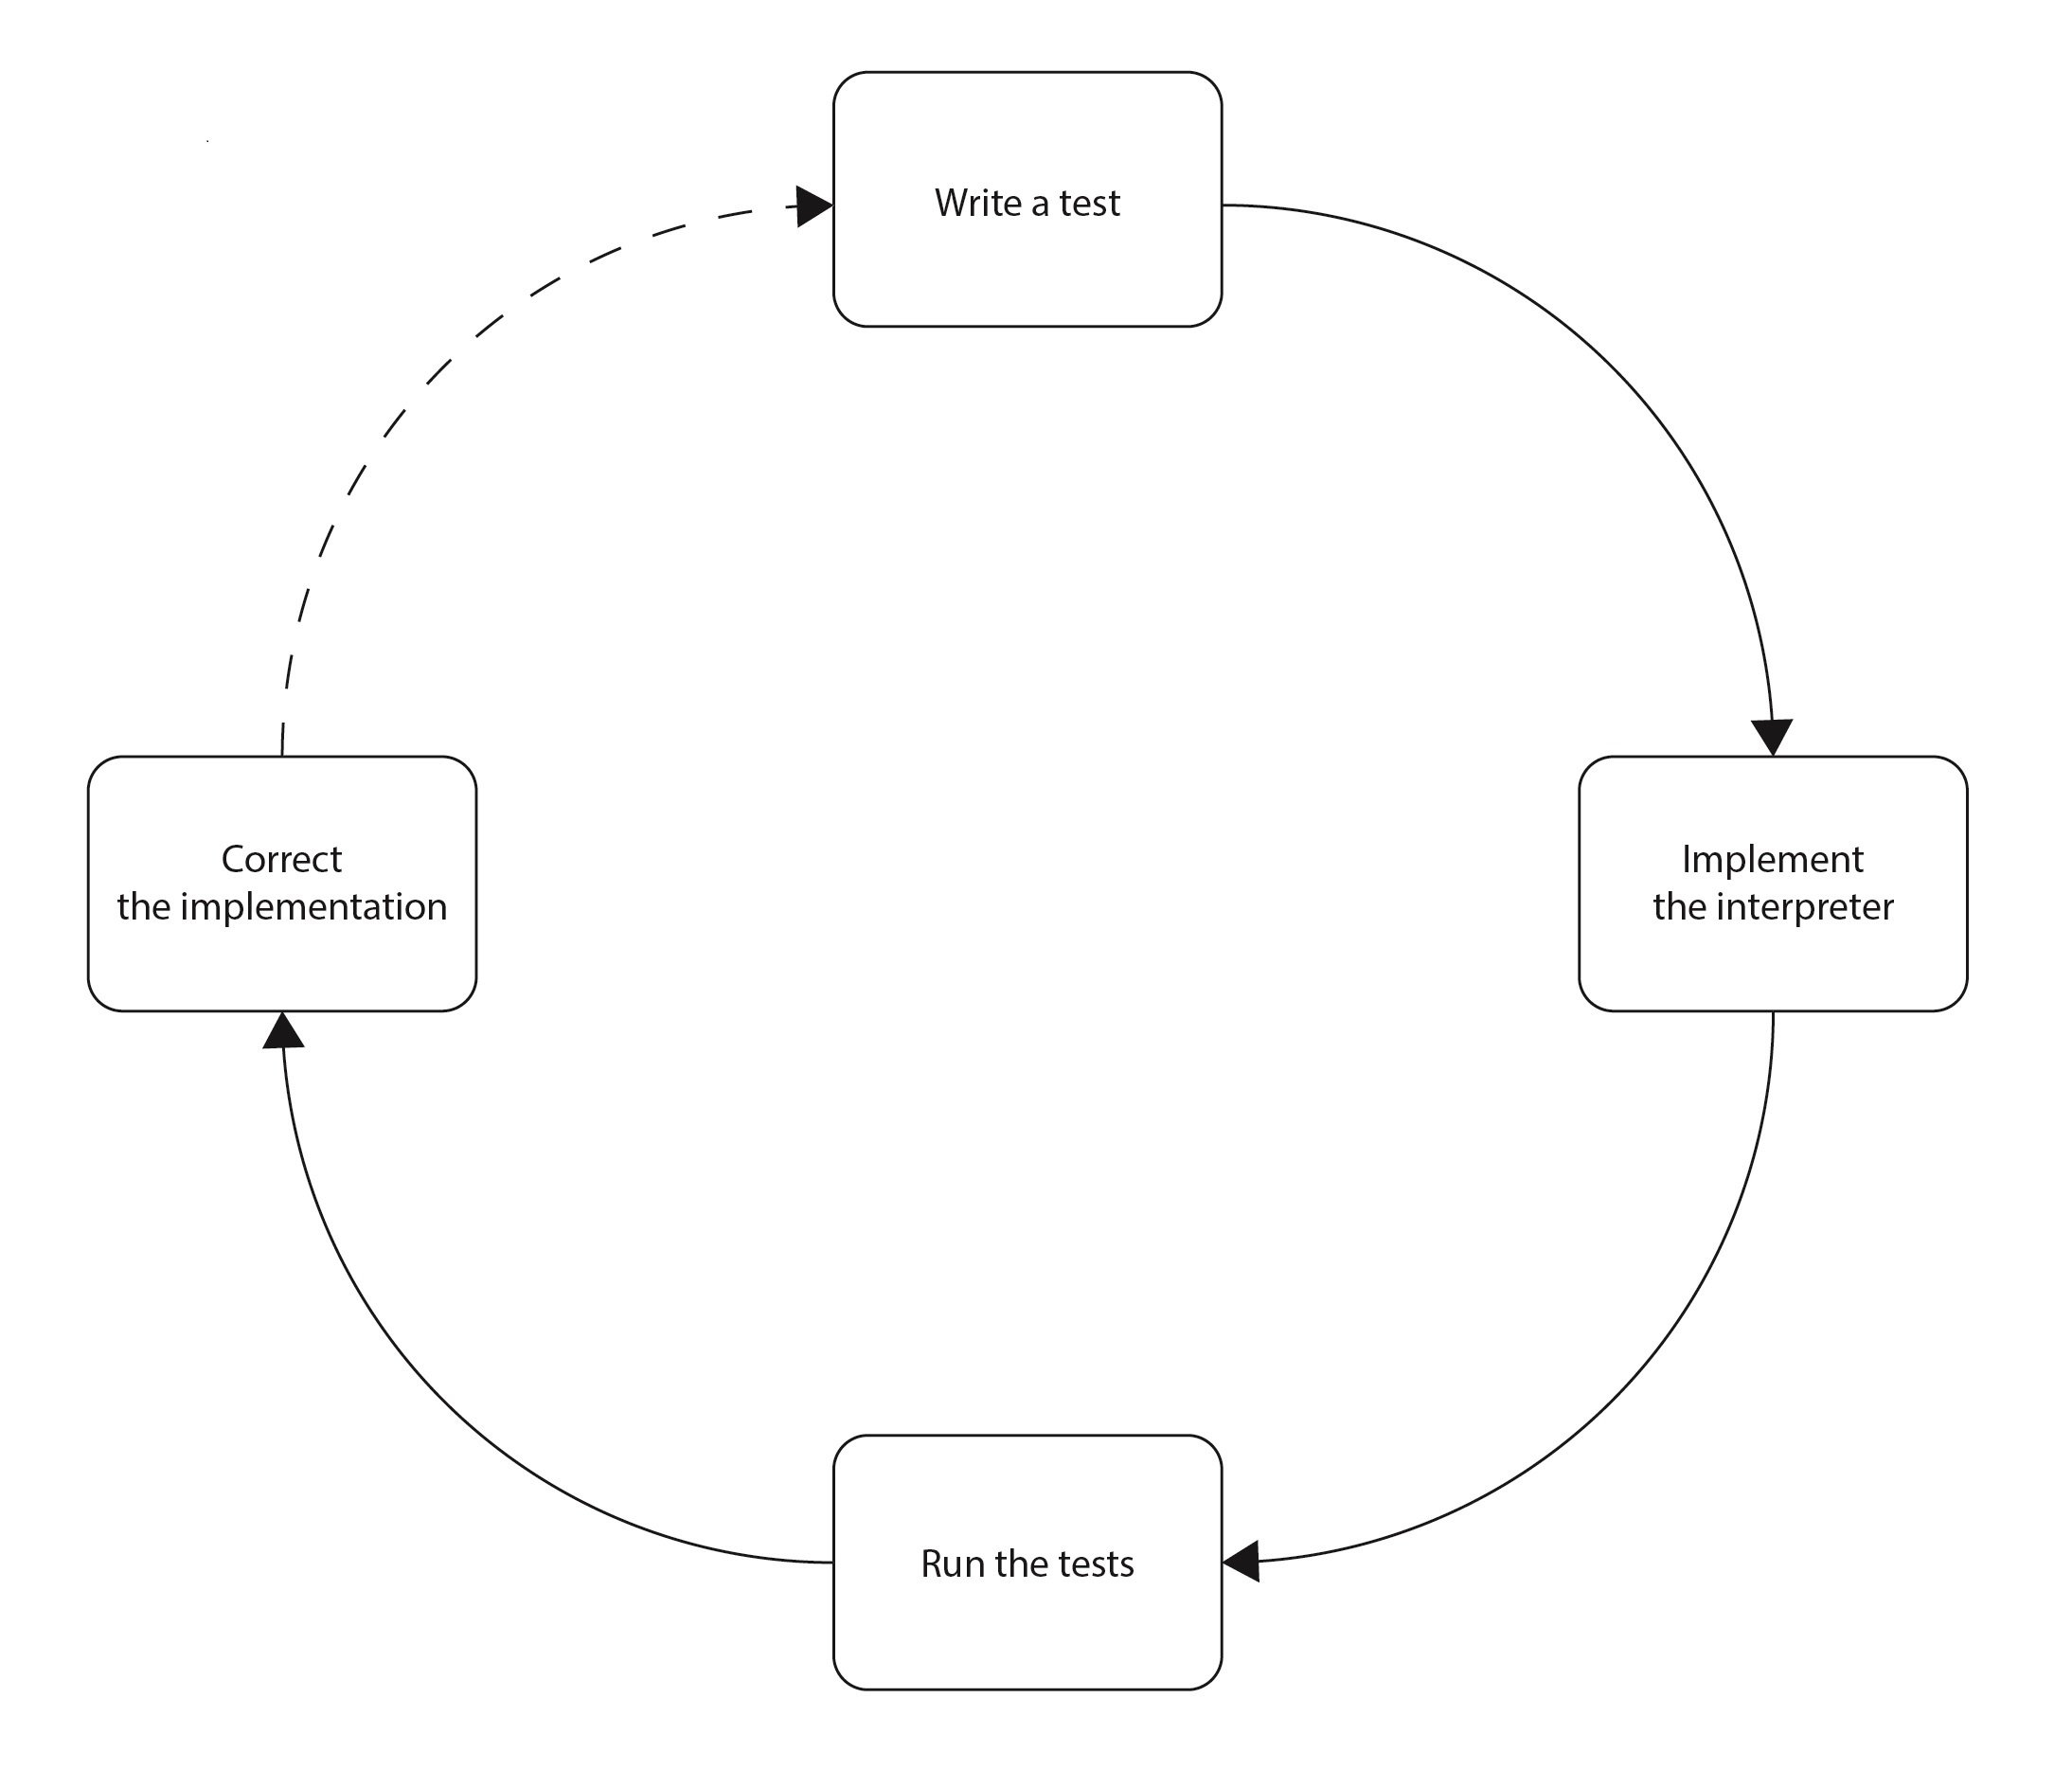
\includegraphics[width=1\textwidth]{process.jpg}
    \centering
    \caption{The process of implementing the interpreter.}
    \label{fig:process}
\end{figure}

\section{The tests}

Potentially, a set of unit tests could be written based on the documentation and the semantics of each instruction. Nevertheless, such a task might be very difficult so another type of tests was used instead. Since there are functioning implementations of the \acrshort{cli}, working of the interpreter can be compared to working of one of such implementations. To be exact, the \texttt{.NET Framework 4.7.2} was selected to write the tests.

Taking into account the abilities of the interpreter, only console programs writing to the standard input, reading from the standard outuput and using the standard error stream are considered proper tests. The vast majority of the tests are written in \texttt{C\#}. Using the \texttt{ildasm} tool provided together with the \texttt{.NET Framework}, the tests can be decompiled to their \acrshort{cil} source code which can be then used as the input file for the interpreter. 

Once a test is prepared, it can be executed using the interpreter and the result of the execution can be compared to the result of the original test program. The result of such a comparison is assumed to be correct when the output produced by the interpreter is the same as the output produced by the original program for the same input. Even though a single test can be potentially executed using an infinite set of different inputs, only a small part is used so that the process is not too time-consuming. In order to make the process as reliable as possible, a set of random inputs is prepared every time the test is executed.

\section{The environment}
\label{sec:environment}

Since repeating the process described above manually might be arduous for bigger numbers of tests, a dedicated system was written separately to automate the procedure. The system is hereinafter called \textit{the tools} or \textit{the environment}. It comprises 2 projects:
\begin{itemize}
	\item{a back-end application,}
	\item{a front-end application.}
\end{itemize}

The back-end application is built using \texttt{ASP.NET Core} which is a modern framework for building Web APIs and applications \cite{littleAsp}. It provides a set of API actions and socket connections that were designed to handle tests, their categories and executions. The application uses a database to store all the data collected so far.

The front-end application was written in \texttt{Typescript} using \texttt{React.js} which is a popular library created for building user interfaces \cite{learningReact}. It is a single-page application that interacts with users and communicates with the back-end application in order to send or receive data.

The tools provide several functionalities described below.

\subsection{Finding tests}

The environment watches the folder provided in the configuration and displays a list of the new tests that have been found. Each of the found tests can be then saved in the database and used to perform various operations. An example of the functionality is shown in figure \ref{fig:tools_find}.

\begin{figure}
	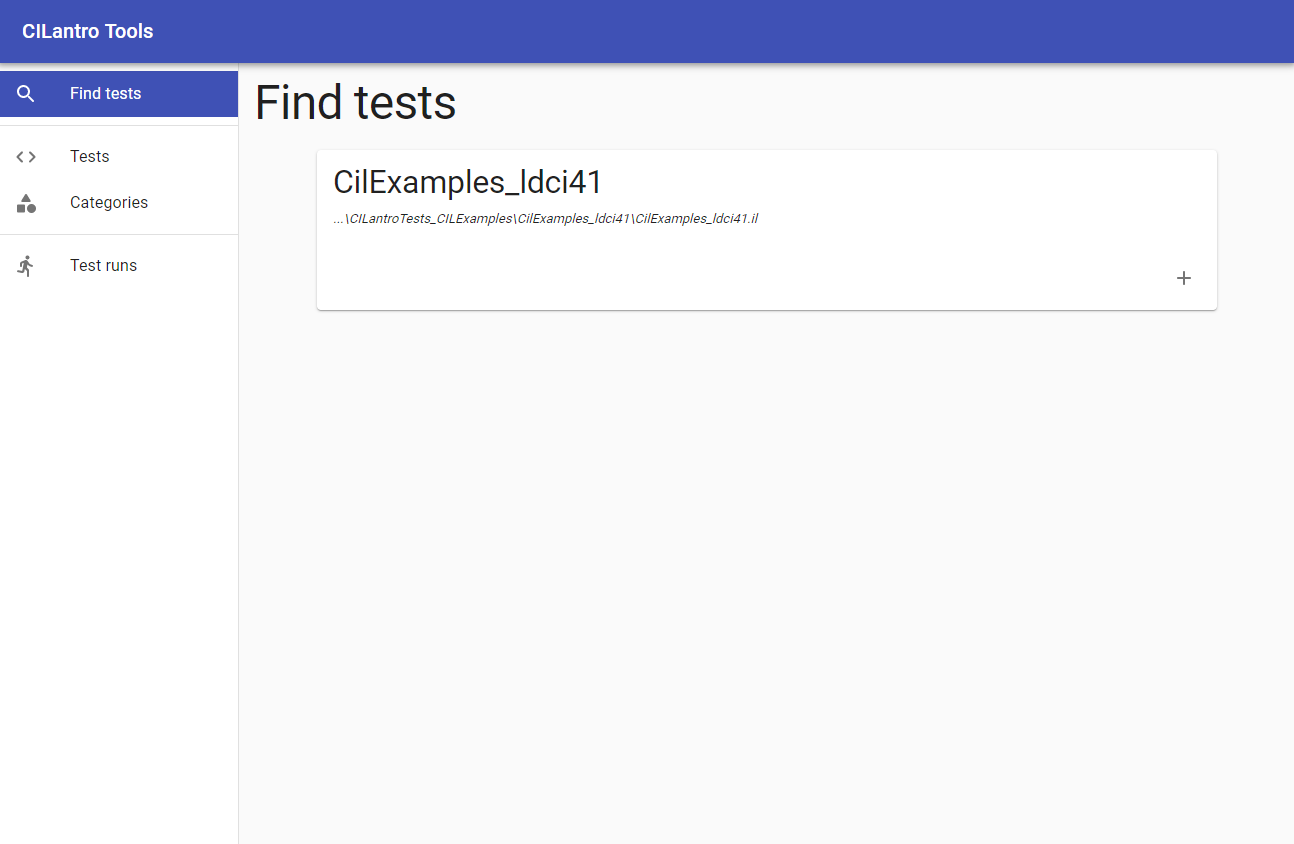
\includegraphics[width=1\textwidth]{tools_find.png}
    \centering
    \caption{The environment - the \textit{Find tests} functionality.}
    \label{fig:tools_find}
\end{figure}

\subsection{Managing categories}

The tools allow the user to define categories and subcategories that can be listed, ordered and filtered. The categories and the subcategories can be then assigned to the tests. The \textit{Categories} page is shown in figure \ref{fig:tools_categories}.

\begin{figure}
	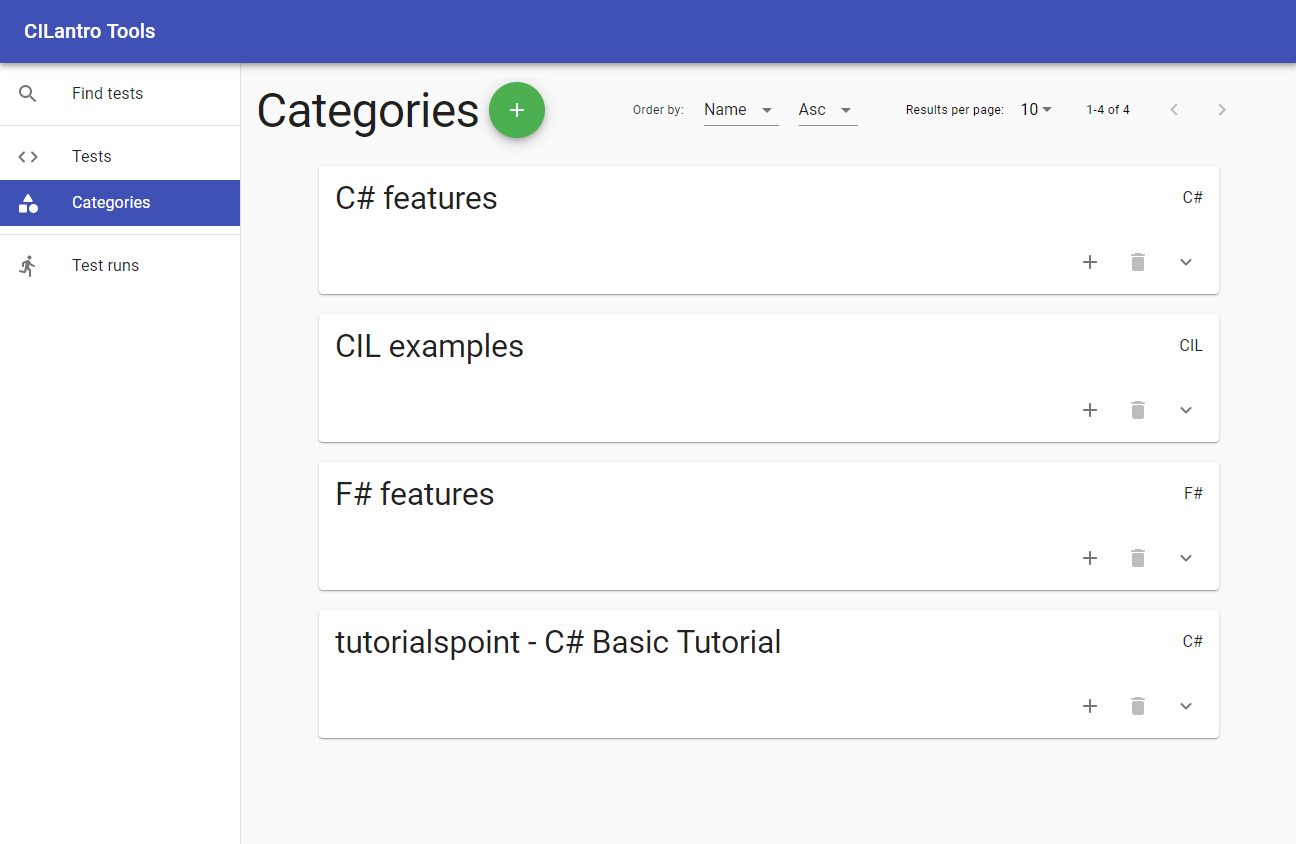
\includegraphics[width=1\textwidth]{tools_categories.png}
    \centering
    \caption{The environment - the \textit{Categories} page.}
    \label{fig:tools_categories}
\end{figure}

\subsection{Managing tests}

The tests can be also listed, ordered and filtered. Each test is presented as a single card of a specific colour which determines the state of the test. If a card is grey, the related test is not configured and needs some additional attention - the card contains a list of tasks to be done in order to configure the test properly. If a card is purple, the corresponding test has been marked as unsupported. If a card is white, the test is ready to be used and run. Additionally, if a test has been already run, the card shows an icon that represents the result of the last run of the test. The \textit{Tests} page is shown in figure \ref{fig:tools_tests}.

\begin{figure}
	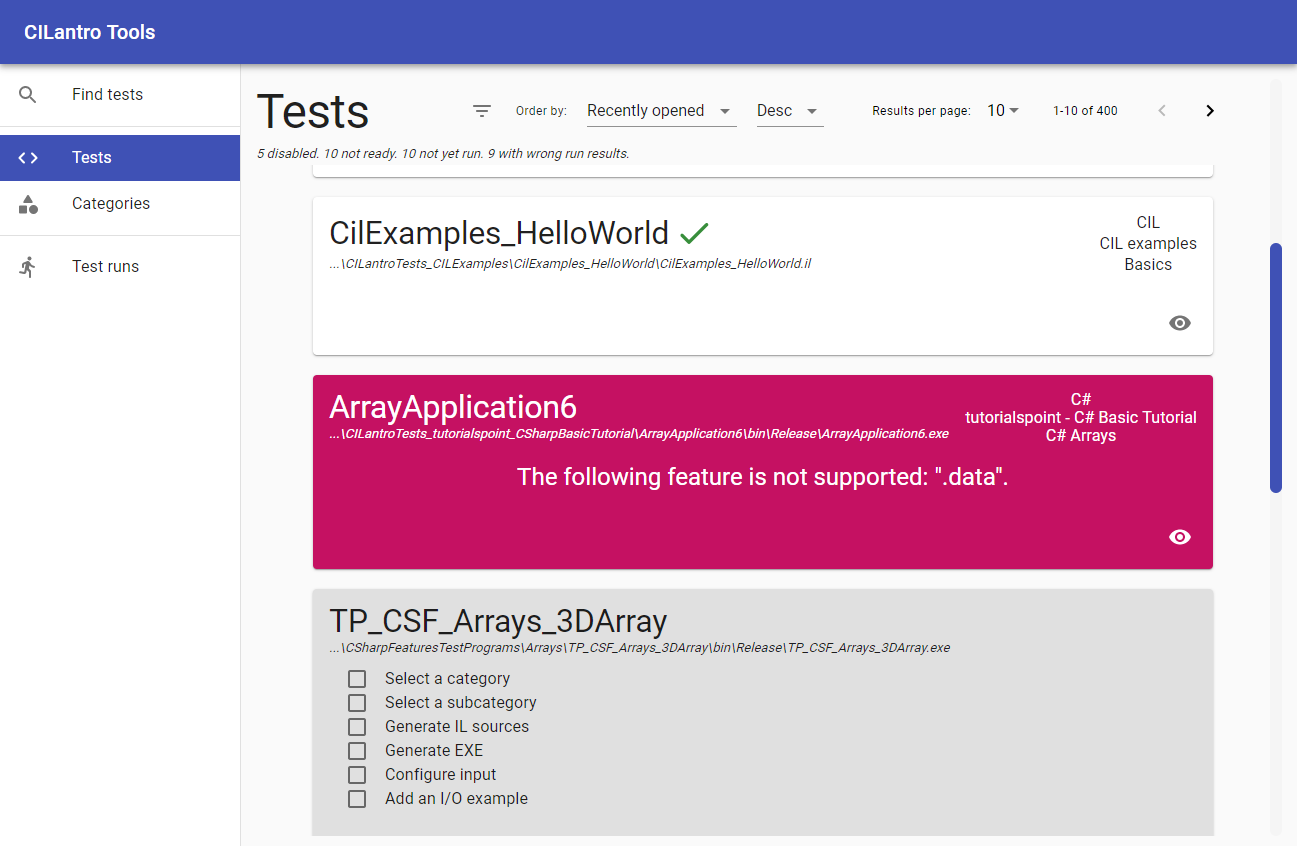
\includegraphics[width=1\textwidth]{tools_tests.png}
    \centering
    \caption{The environment - the \textit{Tests} page.}
    \label{fig:tools_tests}
\end{figure}

\subsection{Managing a single test}

The details of each test defined in the application can be shown on a separate page. The page is divided into the following tabs:
\begin{itemize}
	\item{\texttt{OVERVIEW} - it shows some basic information about the test such as its category and subcategory};
	\item{\texttt{IL SOURCES} - allows the user to display and regenerate the main \texttt{.il} file containing the \acrshort{cil} source code of the test};
	\item{\texttt{EXE} - can be used to compile the source code into an executable file required to execute the test};
	\item{\texttt{I/O} - used for defining example inputs and the pattern of input accepted by the test}.
\end{itemize}

Above the tabs, there is an action area that allows the user to:
\begin{itemize}
	\item{run the original program, the interpreter or both at the same time};
	\item{schedule a test run for the test};
	\item{mark the test as supported or non-supported}.
\end{itemize}

Figure \ref{fig:tools_test} shows a single test page while figure \ref{fig:tools_run_both} presents an example of executing both the original program and the interpreter using the comparison view.

\begin{figure}
	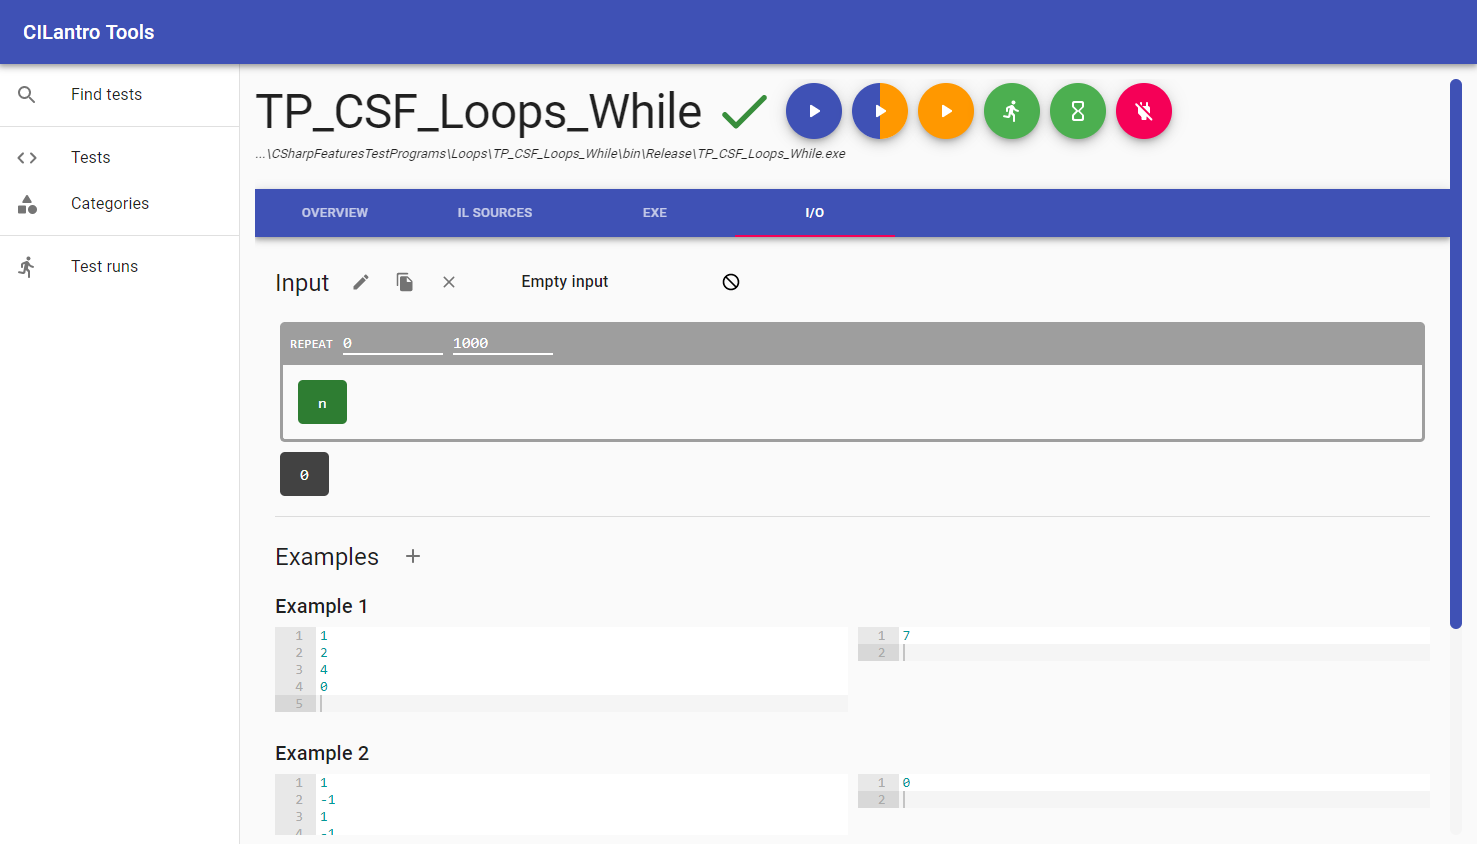
\includegraphics[width=1\textwidth]{tools_test.png}
    \centering
    \caption{The environment - an example test page.}
    \label{fig:tools_test}
\end{figure}

\begin{figure}
	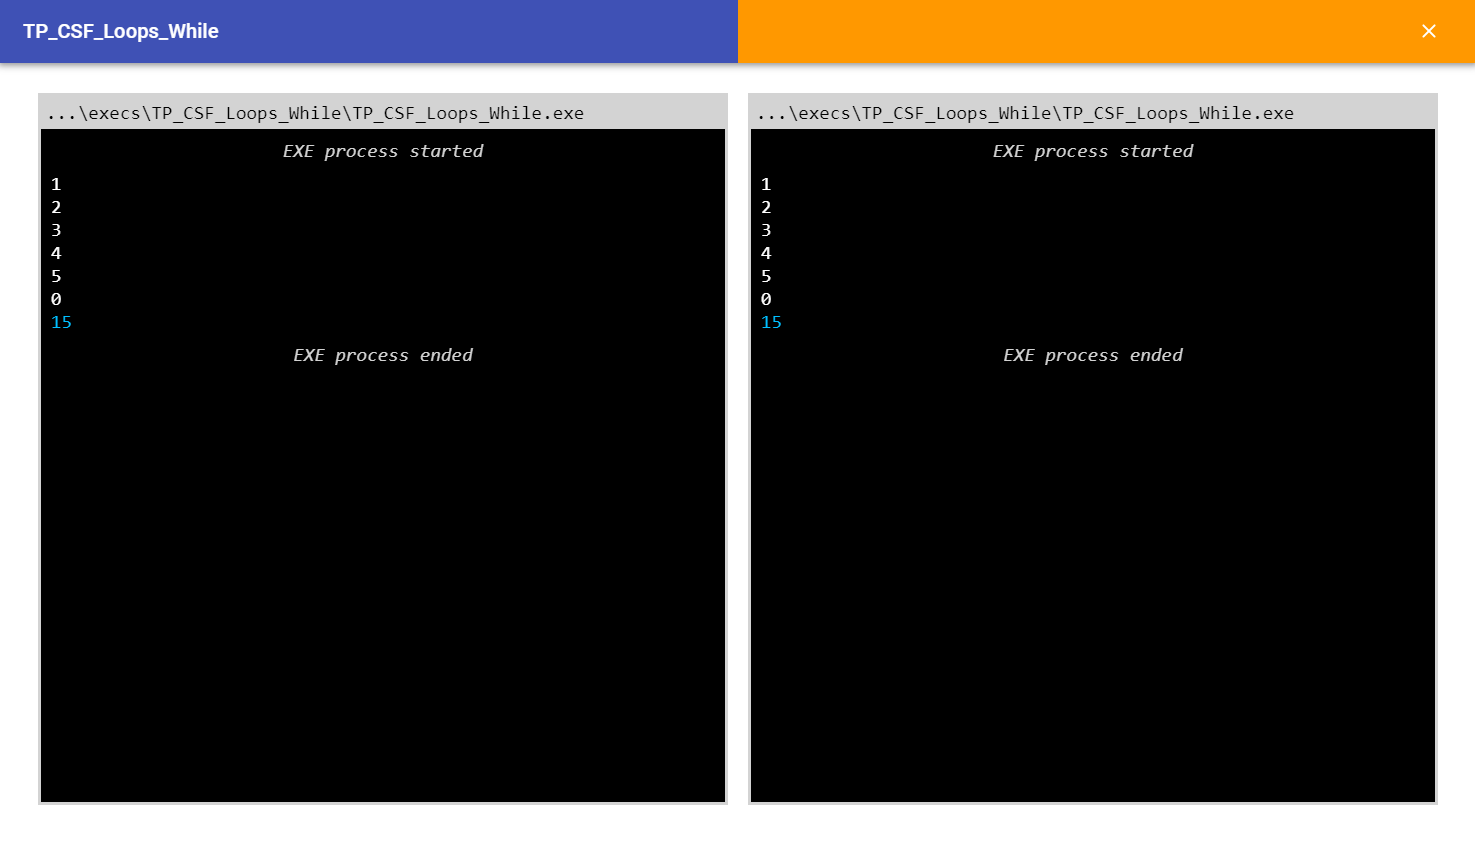
\includegraphics[width=1\textwidth]{tools_run_both.png}
    \centering
    \caption{The environment - running a test in the comparison view.}
    \label{fig:tools_run_both}
\end{figure}

\subsection{Managing test runs}

The test runs can be listed, ordered and filter. A single run is represented by a card of a specific colour. If a card is orange, the corresponding run is being executed at the moment. If a card is red, the run has already ended but its result is wrong. If a card is green, the related run has ended and the result is correct. Each run can be also restarted and the user can display its details.

The page contains two buttons that start a single test run including all the well-configured tests. There are two types of runs: quick and full. A quick run executes each test using only 3 random inputs while a full run uses 100 random inputs for each test. Regardless of the type, each run also executes the tests using the inputs defined in the tools. The \textit{Test runs} page is shown in figure \ref{fig:tools_runs}.

\begin{figure}
	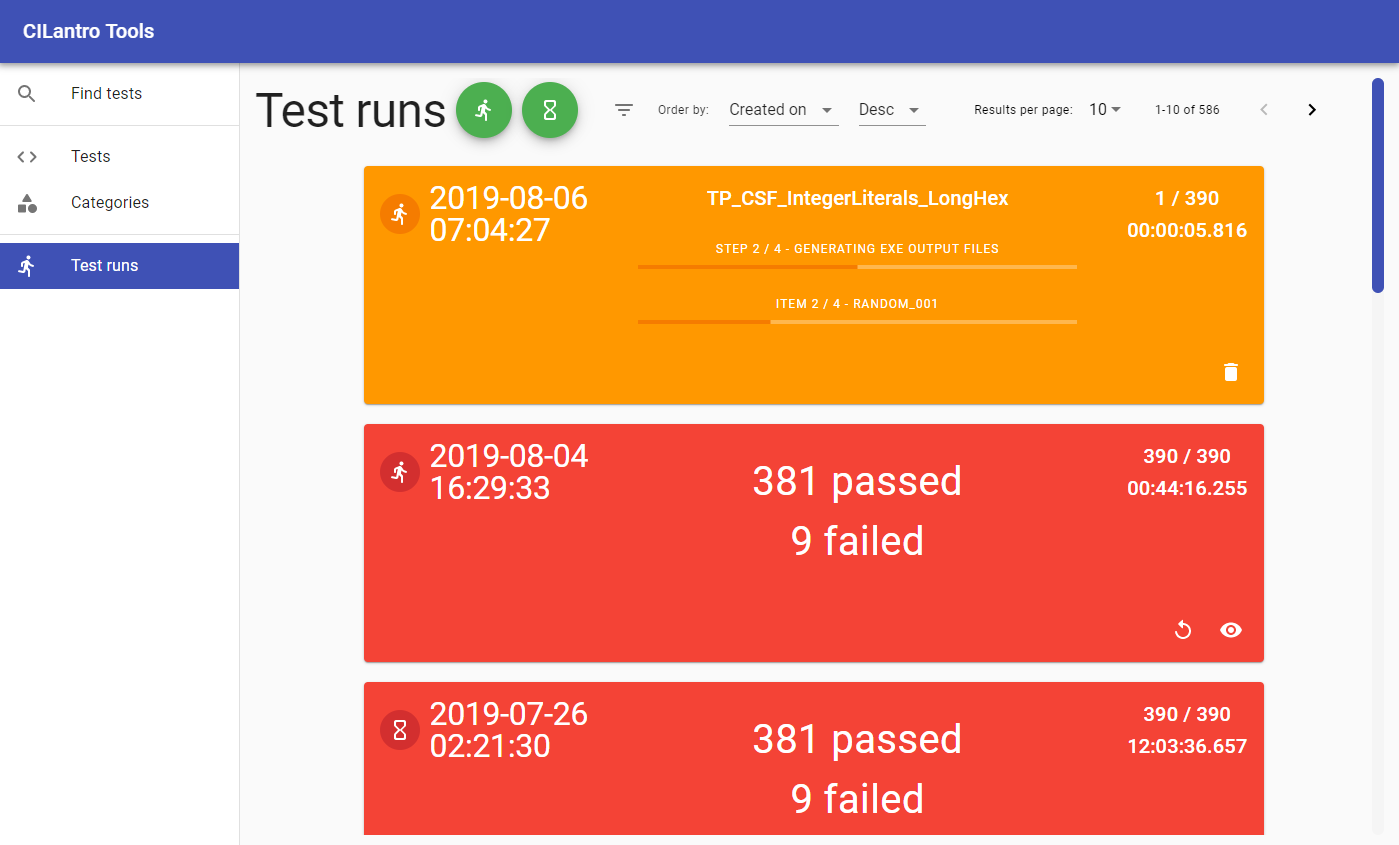
\includegraphics[width=1\textwidth]{tools_runs.png}
    \centering
    \caption{The environment - the \textit{Test runs} page.}
    \label{fig:tools_runs}
\end{figure}

\subsection{Managing a single test run}

Once a test run is finished, its details can be viewed on a separate page. The page contains a card for each test that has been executed within the test run. A card is red if the corresponding test ended with a wrong result and green otherwise. The environment allows the user to open a card and access the details of the executed test. An open card shows a table where each input is represented by a single row containing icons that show the result of each of the following execution phases:
\begin{itemize}
	\item{generating input},
	\item{executing the original program},
	\item{executing the interpreter},
	\item{comparing the results}.
\end{itemize}
Additionally, each row can be also opened in order to see the input and the outputs of the original program and the interpreter. An example of the functionality is shown in figure \ref{fig:tools_run}.

\begin{figure}
	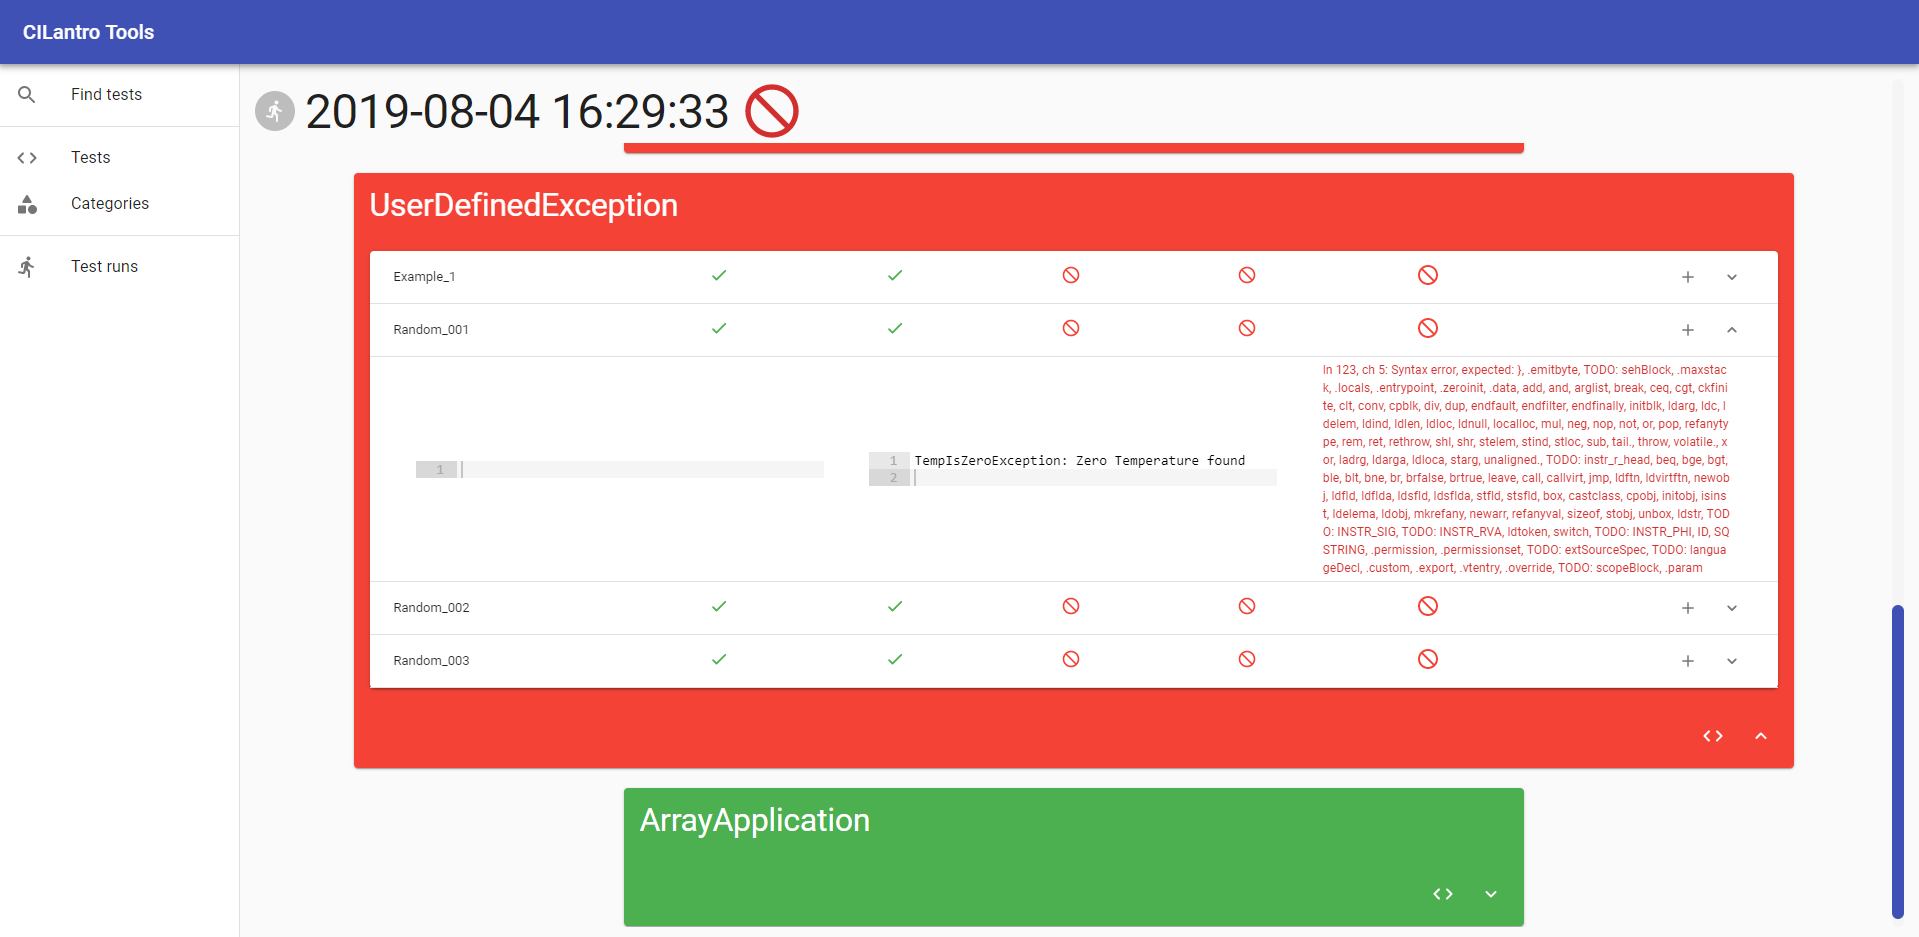
\includegraphics[width=1\textwidth]{tools_run.png}
    \centering
    \caption{The environment - the \textit{Test run} functionality.}
    \label{fig:tools_run}
\end{figure}

\clearpage

%%%%%%%%%%%%%%%%%%%%%%%%%%%%%%%%%%%%%%%%%%%%%%%%%%%%%%%%%%%%%%%%%%%%%%%%%%%%%%%%%%%%%%%%%%
%%%%%%%%%%%%%%%%%%%%%%%%%%%%%%%%%%%%%%%%%%%%%%%%%%%%%%%%%%%%%%%%%%%%%%%%%%%%%%%%%%%%%%%%%%
%%%%%
%%%%%	Results
%%%%%
%%%%%%%%%%%%%%%%%%%%%%%%%%%%%%%%%%%%%%%%%%%%%%%%%%%%%%%%%%%%%%%%%%%%%%%%%%%%%%%%%%%%%%%%%%
%%%%%%%%%%%%%%%%%%%%%%%%%%%%%%%%%%%%%%%%%%%%%%%%%%%%%%%%%%%%%%%%%%%%%%%%%%%%%%%%%%%%%%%%%%

\chapter{Results}
\label{sec:results}

As mentioned, the main goal of the thesis was to implement an interpreter covering as many \acrshort{cil} instructions as possible. The final version of the interpreter fully handles \textbf{101 out of 219} instructions. Moreover, \textbf{17} instructions are partially implemented so they work in some cases but their \texttt{Visit} methods still need to be completed. The details of the \acrshort{cil} instructions set coverage can be found in tables \ref{tab:coverage1} and \ref{tab:coverage2} where:
\begin{itemize}
	\item{$\Circle$ denotes an instruction that is not implemented,}
	\item{$\LEFTcircle$ denotes an instruction that is partially implemented,}
	\item{$\CIRCLE$ denotes an instruction that is fully implemented.}
\end{itemize}

The project itself consists of:
\begin{itemize}
	\item{\textbf{393} source code files (\texttt{.cs}),}
	\item{\textbf{394} \texttt{C\#} classes},
	\item{\textbf{14574} lines of code.}
\end{itemize}

\begin{table}
\begin{center}
	\begin{tabular}{|cc||cc||cc|}
	\hline
\texttt{nop} & \Circle & \texttt{pop} & \CIRCLE & \texttt{ldind.u4} & \Circle \\ \hline
\texttt{break} & \Circle & \texttt{jmp} & \Circle & \texttt{ldind.i8} & \Circle \\ \hline
\texttt{ldarg.0} & \CIRCLE & \texttt{call} & \CIRCLE & \texttt{ldind.i} & \Circle \\ \hline
\texttt{ldarg.1} & \CIRCLE & \texttt{calli} & \Circle & \texttt{ldind.r4} & \Circle \\ \hline
\texttt{ldarg.2} & \CIRCLE & \texttt{ret} & \CIRCLE & \texttt{ldind.r8} & \Circle \\ \hline
\texttt{ldarg.3} & \CIRCLE & \texttt{br.s} & \CIRCLE & \texttt{ldind.ref} & \Circle \\ \hline
\texttt{ldloc.0} & \CIRCLE & \texttt{brfalse.s} & \CIRCLE & \texttt{stind.ref} & \Circle \\ \hline
\texttt{ldloc.1} & \CIRCLE & \texttt{brtrue.s} & \CIRCLE & \texttt{stind.i1} & \Circle \\ \hline
\texttt{ldloc.2} & \CIRCLE & \texttt{beq.s} & \CIRCLE & \texttt{stind.i2} & \Circle \\ \hline
\texttt{ldloc.3} & \CIRCLE & \texttt{bge.s} & \CIRCLE & \texttt{stind.i4} & \LEFTcircle \\ \hline
\texttt{stloc.0} & \CIRCLE & \texttt{bgt.s} & \CIRCLE & \texttt{stind.i8} & \Circle \\ \hline
\texttt{stloc.1} & \CIRCLE & \texttt{ble.s} & \CIRCLE & \texttt{stind.r4} & \Circle \\ \hline
\texttt{stloc.2} & \CIRCLE & \texttt{blt.s} & \CIRCLE & \texttt{stind.r8} & \Circle \\ \hline
\texttt{stloc.3} & \CIRCLE & \texttt{bne.un.s} & \CIRCLE & \texttt{add} & \CIRCLE \\ \hline
\texttt{ldarg.s} & \CIRCLE & \texttt{bge.un.s} & \CIRCLE & \texttt{sub} & \CIRCLE \\ \hline
\texttt{ldarga.s} & \Circle & \texttt{bgt.un.s} & \CIRCLE & \texttt{mul} & \CIRCLE \\ \hline
\texttt{starg.s} & \CIRCLE & \texttt{ble.un.s} & \CIRCLE & \texttt{div} & \CIRCLE \\ \hline
\texttt{ldloc.s} & \CIRCLE & \texttt{blt.un.s} & \CIRCLE & \texttt{div.un} & \CIRCLE \\ \hline
\texttt{ldloca.s} & \LEFTcircle & \texttt{br} & \CIRCLE & \texttt{rem} & \CIRCLE \\ \hline
\texttt{stloc.s} & \CIRCLE & \texttt{brfalse} & \Circle & \texttt{rem.un} & \CIRCLE \\ \hline
\texttt{ldnull} & \Circle & \texttt{brtrue} & \Circle & \texttt{and} & \CIRCLE \\ \hline
\texttt{ldc.i4.m1} & \CIRCLE & \texttt{beq} & \Circle & \texttt{or} & \CIRCLE \\ \hline
\texttt{ldc.i4.0} & \CIRCLE & \texttt{bge} & \Circle & \texttt{xor} & \CIRCLE \\ \hline
\texttt{ldc.i4.1} & \CIRCLE & \texttt{bgt} & \Circle & \texttt{shl} & \CIRCLE \\ \hline
\texttt{ldc.i4.2} & \CIRCLE & \texttt{ble} & \Circle & \texttt{shr} & \CIRCLE \\ \hline
\texttt{ldc.i4.3} & \CIRCLE & \texttt{blt} & \Circle & \texttt{shr.un} & \CIRCLE \\ \hline
\texttt{ldc.i4.4} & \CIRCLE & \texttt{bne.un} & \Circle & \texttt{neg} & \CIRCLE \\ \hline
\texttt{ldc.i4.5} & \CIRCLE & \texttt{bge.un} & \Circle & \texttt{not} & \CIRCLE \\ \hline
\texttt{ldc.i4.6} & \CIRCLE & \texttt{bgt.un} & \Circle & \texttt{conv.i1} & \LEFTcircle \\ \hline
\texttt{ldc.i4.7} & \CIRCLE & \texttt{ble.un} & \Circle & \texttt{conv.i2} & \LEFTcircle \\ \hline
\texttt{ldc.i4.8} & \CIRCLE & \texttt{blt.un} & \Circle & \texttt{conv.i4} & \LEFTcircle \\ \hline
\texttt{ldc.i4.s} & \CIRCLE & \texttt{switch} & \CIRCLE & \texttt{conv.i8} & \LEFTcircle \\ \hline
\texttt{ldc.i4} & \CIRCLE & \texttt{ldind.i1} & \Circle & \texttt{conv.r4} & \LEFTcircle \\ \hline
\texttt{ldc.i8} & \CIRCLE & \texttt{ldind.u1} & \Circle & \texttt{conv.r8} & \LEFTcircle \\ \hline
\texttt{ldc.r4} & \CIRCLE & \texttt{ldind.i2} & \Circle & \texttt{conv.u4} & \Circle \\ \hline
\texttt{ldc.r8} & \CIRCLE & \texttt{ldind.u2} & \Circle & \texttt{conv.u8} & \LEFTcircle \\ \hline
\texttt{dup} & \CIRCLE & \texttt{ldind.i4} & \LEFTcircle & \texttt{callvirt} & \CIRCLE \\ \hline
	\end{tabular}
\caption{The \acrshort{cil} instructions covered by the interpreter (part 1 of 2).}
\label{tab:coverage1}
\end{center}
\end{table}

\begin{table}
\begin{center}
	\begin{tabular}{|cc||cc||cc|}
	\hline
\texttt{cpobj} & \Circle & \texttt{ldelem.i} & \Circle & \texttt{sub.ovf.un} & \Circle \\ \hline
\texttt{ldobj} & \Circle & \texttt{ldelem.r4} & \CIRCLE & \texttt{endfinally} & \Circle \\ \hline
\texttt{ldstr} & \CIRCLE & \texttt{ldelem.r8} & \CIRCLE & \texttt{leave} & \Circle \\ \hline
\texttt{newobj} & \CIRCLE & \texttt{ldelem.ref} & \CIRCLE & \texttt{leave.s} & \Circle \\ \hline
\texttt{castclass} & \Circle & \texttt{stelem.i} & \Circle & \texttt{stind.i} & \Circle \\ \hline
\texttt{isinst} & \LEFTcircle & \texttt{stelem.i1} & \CIRCLE & \texttt{conv.u} & \LEFTcircle \\ \hline
\texttt{conv.r.un} & \LEFTcircle & \texttt{stelem.i2} & \CIRCLE & \texttt{arglist} & \Circle \\ \hline
\texttt{unbox} & \Circle & \texttt{stelem.i4} & \CIRCLE & \texttt{ceq} & \CIRCLE \\ \hline
\texttt{throw} & \Circle & \texttt{stelem.i8} & \CIRCLE & \texttt{cgt} & \CIRCLE \\ \hline
\texttt{ldfld} & \CIRCLE & \texttt{stelem.r4} & \CIRCLE & \texttt{cgt.un} & \CIRCLE \\ \hline
\texttt{ldflda} & \LEFTcircle & \texttt{stelem.r8} & \CIRCLE & \texttt{clt} & \CIRCLE \\ \hline
\texttt{stfld} & \CIRCLE & \texttt{stelem.ref} & \CIRCLE & \texttt{clt.un} & \CIRCLE \\ \hline
\texttt{ldsfld} & \CIRCLE & \texttt{ldelem} & \CIRCLE & \texttt{ldftn} & \Circle \\ \hline
\texttt{ldsflda} & \Circle & \texttt{stelem} & \CIRCLE & \texttt{ldvirtftn} & \Circle \\ \hline
\texttt{stsfld} & \CIRCLE & \texttt{unbox.any} & \CIRCLE & \texttt{ldarg} & \Circle \\ \hline
\texttt{stobj} & \Circle & \texttt{conv.ovf.i1} & \Circle & \texttt{ldarga} & \Circle \\ \hline
\texttt{conv.ovf.i1.un} & \Circle & \texttt{conv.ovf.u1} & \Circle & \texttt{starg} & \Circle \\ \hline
\texttt{conv.ovf.i2.un} & \Circle & \texttt{conv.ovf.i2} & \Circle & \texttt{ldloc} & \Circle \\ \hline
\texttt{conv.ovf.i4.un} & \Circle & \texttt{conv.ovf.u2} & \Circle & \texttt{ldloca} & \Circle \\ \hline
\texttt{conv.ovf.i8.un} & \Circle & \texttt{conv.ovf.i4} & \Circle & \texttt{stloc} & \Circle \\ \hline
\texttt{conv.ovf.u1.un} & \Circle & \texttt{conv.ovf.u4} & \Circle & \texttt{localloc} & \Circle \\ \hline
\texttt{conv.ovf.u2.un} & \Circle & \texttt{conv.ovf.i8} & \Circle & \texttt{endfilter} & \Circle \\ \hline
\texttt{conv.ovf.u4.un} & \Circle & \texttt{conv.ovf.u8} & \Circle & \texttt{unaligned.} & \Circle \\ \hline
\texttt{conv.ovf.u8.un} & \Circle & \texttt{refanyval} & \Circle & \texttt{volatile.} & \Circle \\ \hline
\texttt{conv.ovf.i.un} & \Circle & \texttt{ckfinite} & \Circle & \texttt{tail.} & \Circle \\ \hline
\texttt{conv.ovf.u.un} & \Circle & \texttt{mkrefany} & \Circle & \texttt{Initobj} & \CIRCLE \\ \hline
\texttt{box} & \CIRCLE & \texttt{ldtoken} & \LEFTcircle & \texttt{constrained.} & \Circle \\ \hline
\texttt{newarr} & \CIRCLE & \texttt{conv.u2} & \LEFTcircle & \texttt{cpblk} & \Circle \\ \hline
\texttt{ldlen} & \CIRCLE & \texttt{conv.u1} & \LEFTcircle & \texttt{initblk} & \Circle \\ \hline
\texttt{ldelema} & \Circle & \texttt{conv.i} & \Circle & \texttt{no.} & \Circle \\ \hline
\texttt{ldelem.i1} & \CIRCLE & \texttt{conv.ovf.i} & \Circle & \texttt{rethrow} & \Circle \\ \hline
\texttt{ldelem.u1} & \CIRCLE & \texttt{conv.ovf.u} & \Circle & \texttt{sizeof} & \Circle \\ \hline
\texttt{ldelem.i2} & \CIRCLE & \texttt{add.ovf} & \Circle & \texttt{Refanytype} & \Circle \\ \hline
\texttt{ldelem.u2} & \CIRCLE & \texttt{add.ovf.un} & \Circle & \texttt{readonly.} & \Circle \\ \hline
\texttt{ldelem.i4} & \CIRCLE & \texttt{mul.ovf} & \Circle &  &  \\ \hline
\texttt{ldelem.u4} & \CIRCLE & \texttt{mul.ovf.un} & \Circle &  &  \\ \hline
\texttt{ldelem.i8} & \CIRCLE & \texttt{sub.ovf} & \Circle &  &  \\ \hline
	\end{tabular}
\caption{The \acrshort{cil} instructions covered by the interpreter (part 2 of 2).}
\label{tab:coverage2}
\end{center}
\end{table}

While working on the interpreter, a total number of \textbf{408} tests were used where:
\begin{itemize}
	\item{\textbf{328} tests were written manually using mainly \texttt{C\#} but also \texttt{F\#} and the \acrshort{cil} itself;}
	\item{\textbf{80} tests were adopted from \cite{tutorialspoint};}
	\item{\textbf{384} tests were successfully handled by the interpreter;}
	\item{\textbf{more than 14000} lines of code were produced for the manually created tests.}
\end{itemize}

The environment presented in section \ref{sec:environment} was written using:
\begin{itemize}
	\item{\textbf{10348} lines of code for the back-end application,}
	\item{\textbf{8276} lines of code for the front-end application.}
\end{itemize}

\section{Performance}
\label{sec:performance}

Although performance was not a part of the thesis, 3 special tests were written in order to compare the performance of the interpreter to the standard \texttt{.NET Framework 4.7.2} implementation. Each of the charts included in this section presents results in the same manner. Each input data was used 5 times and a chart presents the average execution time in milliseconds. The left column corresponds to the original program while the right one relates to the interpreter. The logarithmic scale was used for each chart.

The first program computes the $n$-th Fibonacci number using the standard recursive formula. It relates to figure \ref{fig:fibonacci_chart}. The second test computes the Ackermann function using the recursive formula again and corresponds to figure \ref{fig:ackermann_chart}. The last performance test simply writes out the first $n$ natural numbers and its results are presented in figure \ref{fig:natural_chart}.

\begin{figure}
	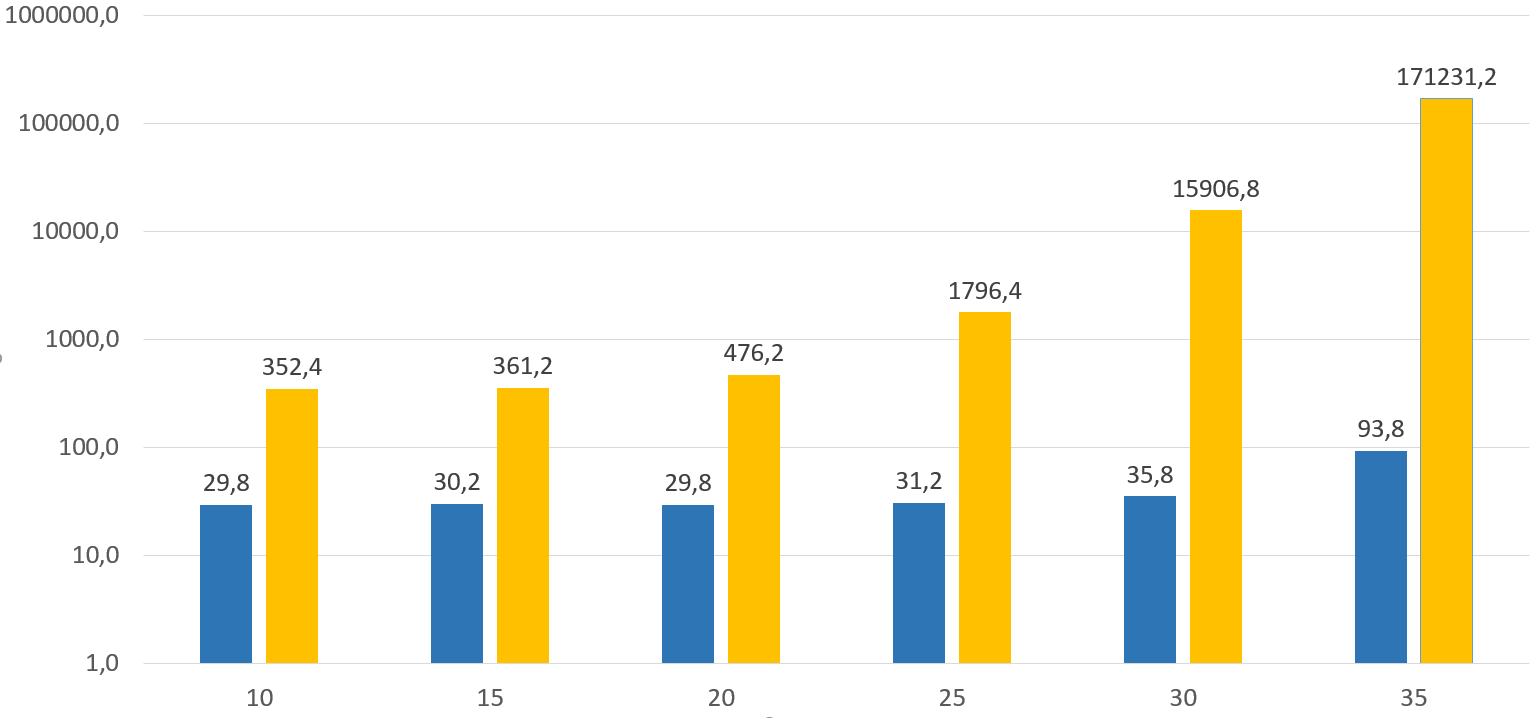
\includegraphics[width=1\textwidth]{fibonacci_chart.png}
    \centering
    \caption{Average execution time of the Fibonacci test program.}
    \label{fig:fibonacci_chart}
\end{figure}

\begin{figure}
	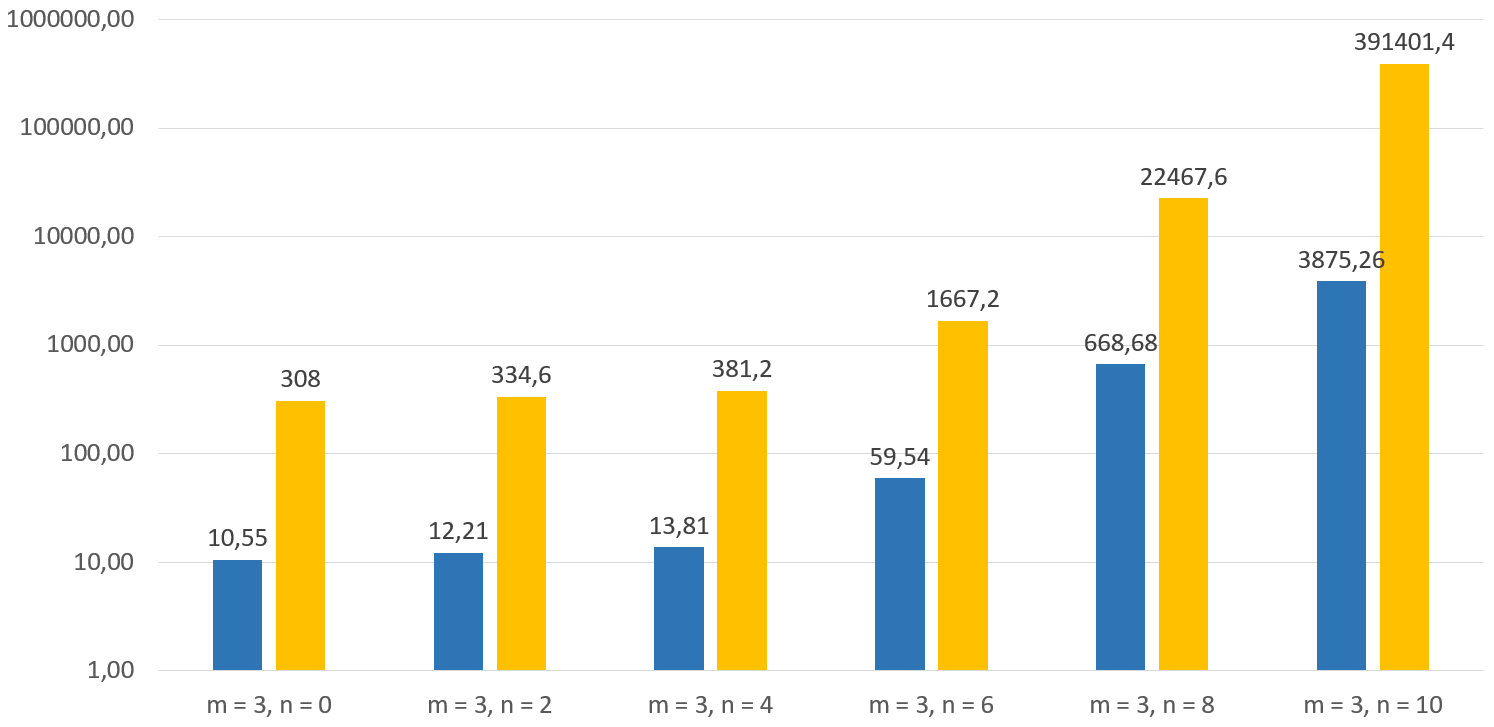
\includegraphics[width=1\textwidth]{ackermann_chart.png}
    \centering
    \caption{Average execution time of the Ackermann function test program.}
    \label{fig:ackermann_chart}
\end{figure}

\begin{figure}
	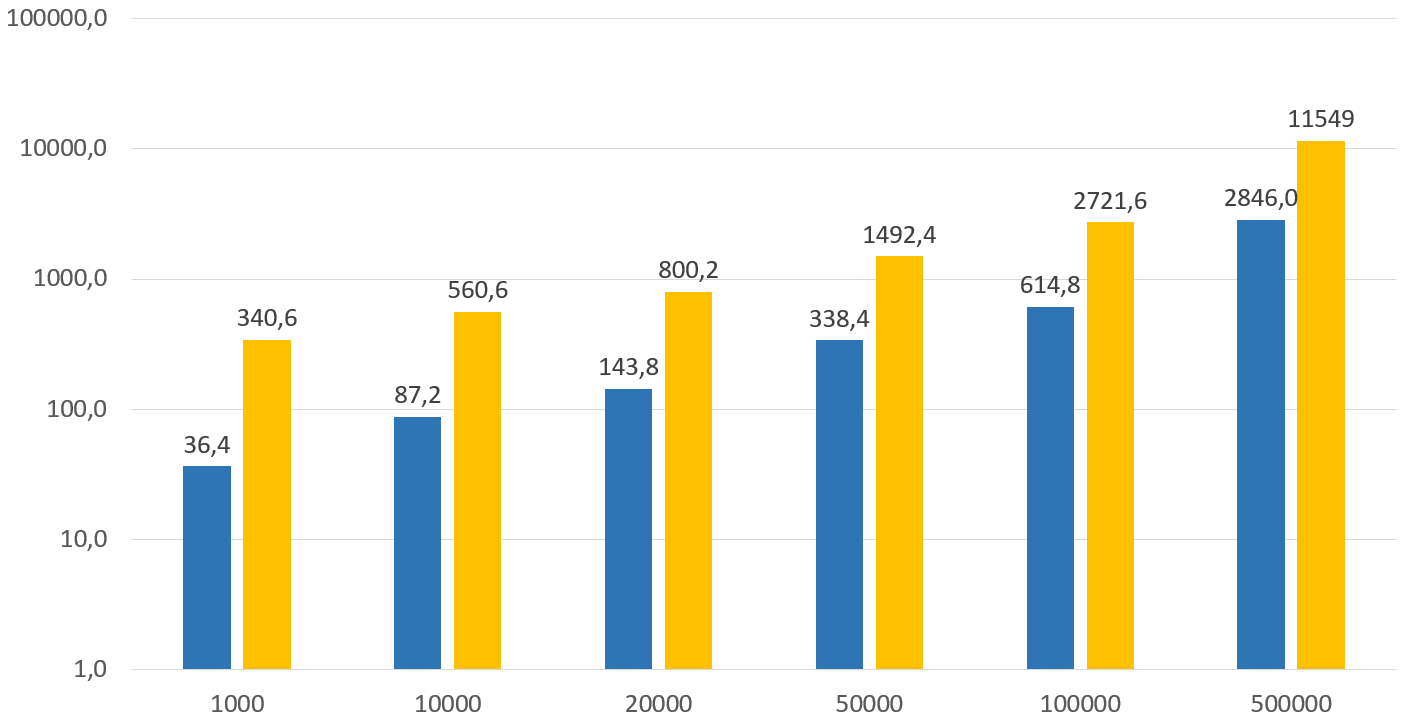
\includegraphics[width=1\textwidth]{natural_chart.png}
    \centering
    \caption{Average execution time of the natural numbers writer.}
    \label{fig:natural_chart}
\end{figure}

As shown in the figures, the interpreter seems to work much slower than the original test programs. However, it might have been anticipated. There are several reasons that could explain the performance gap between the two:
\begin{itemize}
	\item{The interpreter works directly on the source code while the \texttt{.NET Framework} operates on compiled versions of programs.}
	\item{The interpreter is written in \texttt{C\#} which is itself executed by the framework.}
	\item{The implementation of the interpreter is simplified and could be potentially improved as shown in section \ref{sec:future_work}.}
\end{itemize}

\clearpage

%%%%%%%%%%%%%%%%%%%%%%%%%%%%%%%%%%%%%%%%%%%%%%%%%%%%%%%%%%%%%%%%%%%%%%%%%%%%%%%%%%%%%%%%%%
%%%%%%%%%%%%%%%%%%%%%%%%%%%%%%%%%%%%%%%%%%%%%%%%%%%%%%%%%%%%%%%%%%%%%%%%%%%%%%%%%%%%%%%%%%
%%%%%
%%%%%	Conclusions & future work
%%%%%
%%%%%%%%%%%%%%%%%%%%%%%%%%%%%%%%%%%%%%%%%%%%%%%%%%%%%%%%%%%%%%%%%%%%%%%%%%%%%%%%%%%%%%%%%%
%%%%%%%%%%%%%%%%%%%%%%%%%%%%%%%%%%%%%%%%%%%%%%%%%%%%%%%%%%%%%%%%%%%%%%%%%%%%%%%%%%%%%%%%%%

\chapter{Conclusions and future work}
\label{sec:conclusions}

Only a few programming languages are well-described and standardised. The \acrshort{cil} with its formal documentation seemed to be an ideal candidate for investigating its semantics and trying to build an interpreter. Nevertheless, the standard is sometimes deficient in important details and its contents have not been updated for several years.
Additionally, the \acrshort{cil} itself introduces various features and approaches and its instruction set is quite big.

Taken all together, building an interpreter of a complex and modern programming language is a very time-consuming undertaking. There are many details that need to be taken into consideration. Some solutions implemented at the first attempt turn out to be insufficient or inadequate hence they need to be rewritten all over again.

Furthermore, building an interpreter has to be done simultaneously with several different tasks. It is indeed a process that involves additional work such as creating tests, taking care of compatibility and investigating defects. For instance, the environment built as a part of the thesis required a big effort but was crucial in terms of testing the solution.

To sum up, the thesis and the project explain why there is often a large number of developers, engineers, testers and other people involved in the process of building and improving modern and valuable programming languages.

\section{Future work}
\label{sec:future_work}

There are several areas that could be potentially improved or completed in terms of the interpreter:
\begin{itemize}
	\item{The whole \acrshort{cil} instruction set could be covered.}
	\item{The interpreter supports console programs only. The only interaction with the user can be arranged through the standard input, output and error streams. One could extend this model and try to support different types of communication with end users.}
	\item{No external code is interpreted at the moment. The interpreter uses a \texttt{C\#} mechanism known as \textit{reflection} in order to call and execute methods from external assemblies.}
	\item{As mentioned in section \ref{sec:managedMemory}, the memory operations are currently simulated which results in some limitations. For example, the unmanaged memory cannot be accessed by the interpreted program, it also depends on the \texttt{C\#} memory management. A full implementation could involve a completely new approach for the memory.}
	\item{No garbage collector is implemented so values remain in the memory until the very end of the program.}
	\item{There is no support for multithreading or asynchronous operations.}
	\item{The algorithm described in section \ref{sec:codeVerifiability} could be implemented and involved in the whole process of interpreting. For now, the interpreter cannot verify the input code thus only correct programs are allowed.}
	\item{As shown in section \ref{sec:performance}, the performance of the interpreter could be possibly improved.}
\end{itemize}

\clearpage

%%%%%%%%%%%%%%%%%%%%%%%%%%%%%%%%%%%%%%%%%%%%%%%%%%%%%%%%%%%%%%%%%%%%%%%%%%%%%%%%%%%%%%%%%%
%%%%%%%%%%%%%%%%%%%%%%%%%%%%%%%%%%%%%%%%%%%%%%%%%%%%%%%%%%%%%%%%%%%%%%%%%%%%%%%%%%%%%%%%%%
%%%%%
%%%%%	Bibliography
%%%%%
%%%%%%%%%%%%%%%%%%%%%%%%%%%%%%%%%%%%%%%%%%%%%%%%%%%%%%%%%%%%%%%%%%%%%%%%%%%%%%%%%%%%%%%%%%
%%%%%%%%%%%%%%%%%%%%%%%%%%%%%%%%%%%%%%%%%%%%%%%%%%%%%%%%%%%%%%%%%%%%%%%%%%%%%%%%%%%%%%%%%%

\renewcommand{\refname}{Bibliography}

\bibliography{mgr}{}
\bibliographystyle{unsrt}

%%%%%%%%%%%%%%%%%%%%%%%%%%%%%%%%%%%%%%%%%%%%%%%%%%%%%%%%%%%%%%%%%%%%%%%%%%%%%%%%%%%%%%%%%%
%%%%%%%%%%%%%%%%%%%%%%%%%%%%%%%%%%%%%%%%%%%%%%%%%%%%%%%%%%%%%%%%%%%%%%%%%%%%%%%%%%%%%%%%%%
%%%%%
%%%%%	End document
%%%%%
%%%%%%%%%%%%%%%%%%%%%%%%%%%%%%%%%%%%%%%%%%%%%%%%%%%%%%%%%%%%%%%%%%%%%%%%%%%%%%%%%%%%%%%%%%
%%%%%%%%%%%%%%%%%%%%%%%%%%%%%%%%%%%%%%%%%%%%%%%%%%%%%%%%%%%%%%%%%%%%%%%%%%%%%%%%%%%%%%%%%%

\end{document}